\documentclass[9pt]{article}
\usepackage[english]{babel}
\usepackage{amsmath,amsthm}
\usepackage{amsfonts}
\usepackage{graphicx}
\usepackage[margin=0.2in]{geometry}
\newcommand{\setlinespacing}[1]{\setlength{\baselineskip}{#1 \defbaselineskip}}
\newcommand{\doublespacing}{\setlength{\baselineskip}{2.0 \defbaselineskip}}
\newcommand{\singlespacing}{\setlength{\baselineskip}{\defbaselineskip}}
\newcommand{\A}{{\cal A}}
\newcommand{\h}{{\cal H}}
\newcommand{\s}{{\cal S}}
\newcommand{\W}{{\cal W}}
\newcommand{\BH}{\mathbf B(\cal H)}
\newcommand{\KH}{\cal  K(\cal H)}
\newcommand{\Real}{\mathbb R}
\newcommand{\Complex}{\mathbb C}
\newcommand{\Field}{\mathbb F}
\newcommand{\RPlus}{[0,\infty)}
\newcommand{\norm}[1]{\left\Vert#1\right\Vert}
\newcommand{\essnorm}[1]{\norm{#1}_{\text{\rm\normalshape ess}}}
\newcommand{\abs}[1]{\left\vert#1\right\vert}
\newcommand{\set}[1]{\left\{#1\right\}}
\newcommand{\seq}[1]{\left<#1\right>}
\newcommand{\eps}{\varepsilon}
\newcommand{\To}{\longrightarrow}
\newcommand{\RE}{\operatorname{Re}}
\newcommand{\IM}{\operatorname{Im}}
\newcommand{\Poly}{{\cal{P}}(E)}
\newcommand{\EssD}{{\cal{D}}}
\newcommand{\field}[1]{\mathbb{#1}}
\newcommand{\C}{\field{C}}
\newcommand{\R}{\field{R}}
\newcommand{\script}[1]{\mathcal{#1}}
\newcommand{\fall}{\; \forall \;}
\newcommand{\exts}{\; \exists \;}
\newcommand{\mbf}[1]{\mathbf{#1}}
\newcommand{\binomial}[2]{\biggl( \begin{array}{c}  #1 \\ #2  \\ \end{array} \biggr) }
\newcommand{\fderiv}[2]{ \frac{d}{ d #1} \: #2}
\newcommand{\sderiv}[2]{ \frac{d^2}{ d^2 #1} \: #2}
\newcommand{\pfderiv}[2]{ \frac{\partial}{ \partial #1} \: #2}
\newcommand{\psderiv}[2]{ \frac{\partial^2}{ \partial^2 #1} \: #2}
\newcommand{\mat}[1]{\mathbf{#1}}
\DeclareSymbolFont{AMSb}{U}{msb}{m}{n}
\DeclareMathSymbol{\dblz}{\mathalpha}{AMSb}{"5A}
\DeclareMathSymbol{\dblr}{\mathalpha}{AMSb}{"52}
\DeclareMathSymbol{\dblt}{\mathalpha}{AMSb}{"54}
\DeclareMathSymbol{\dblq}{\mathalpha}{AMSb}{"51}
\DeclareMathSymbol{\dbln}{\mathalpha}{AMSb}{"4E}
\DeclareMathSymbol{\dblf}{\mathalpha}{AMSb}{"46}
\DeclareMathSymbol{\dblc}{\mathalpha}{AMSb}{"43}
\DeclareMathSymbol{\dbld}{\mathalpha}{AMSb}{"44}
\theoremstyle{plain}
\newtheorem{thm}{Theorem}[section]
\newtheorem{cor}[thm]{Corollary}
\newtheorem{lem}[thm]{Lemma}
\newtheorem{prop}[thm]{Proposition}
\theoremstyle{definition}
\newtheorem{defn}{Definition}[section]
\theoremstyle{remark}
\newtheorem{rem}{Remark}[section]
\numberwithin{equation}{section}
\renewcommand{\theequation}{\thesection.\arabic{equation}}
\begin{document}
\title{Regression of KL Software Distribution   }
\author{KL Software Libraries}
\date{Mon May 12 15:15:05 2014
}
\maketitle
\textbf{ KL Library test output.  This LaTex file and the associated diagrams are produced by the KL software libraries.}
QueryPerformanceCounter  =  1.6651
\subsubsection{Iterated Exponential Filtering }
$\mu_1 =0.0930085$
$\mu_2 =0.725636$
$\mu_3 =0.0110119$
$\mu_4 =2.17812$
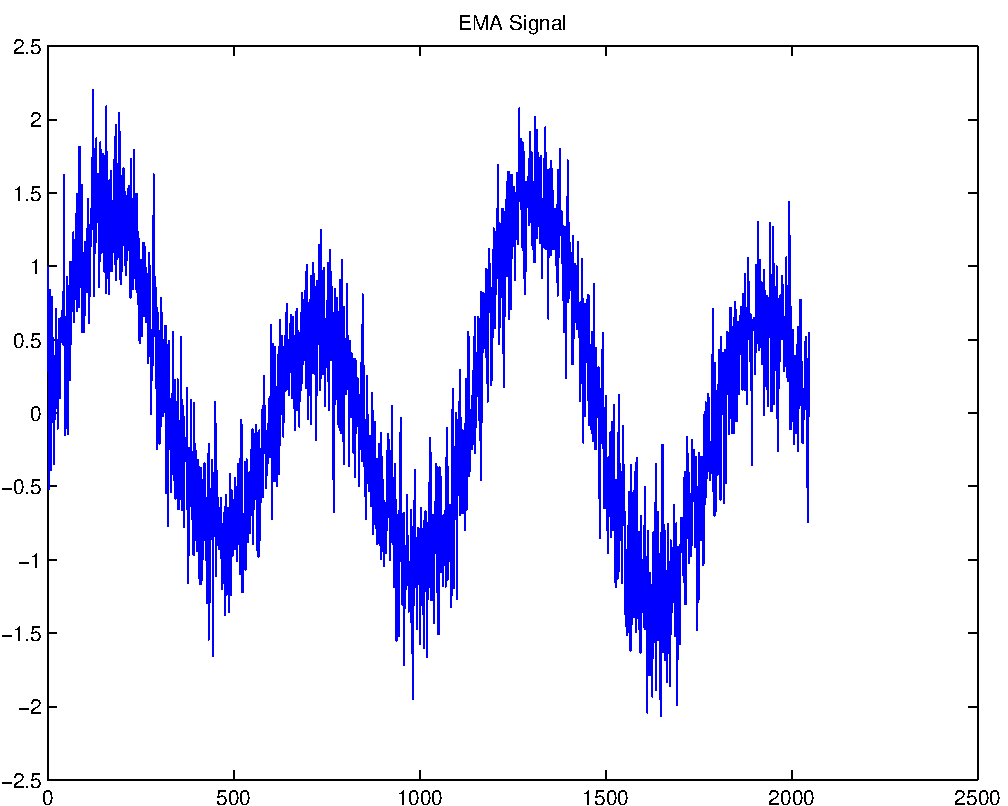
\includegraphics[width=10.0cm,height=10.0cm]{EMA_signal.pdf}

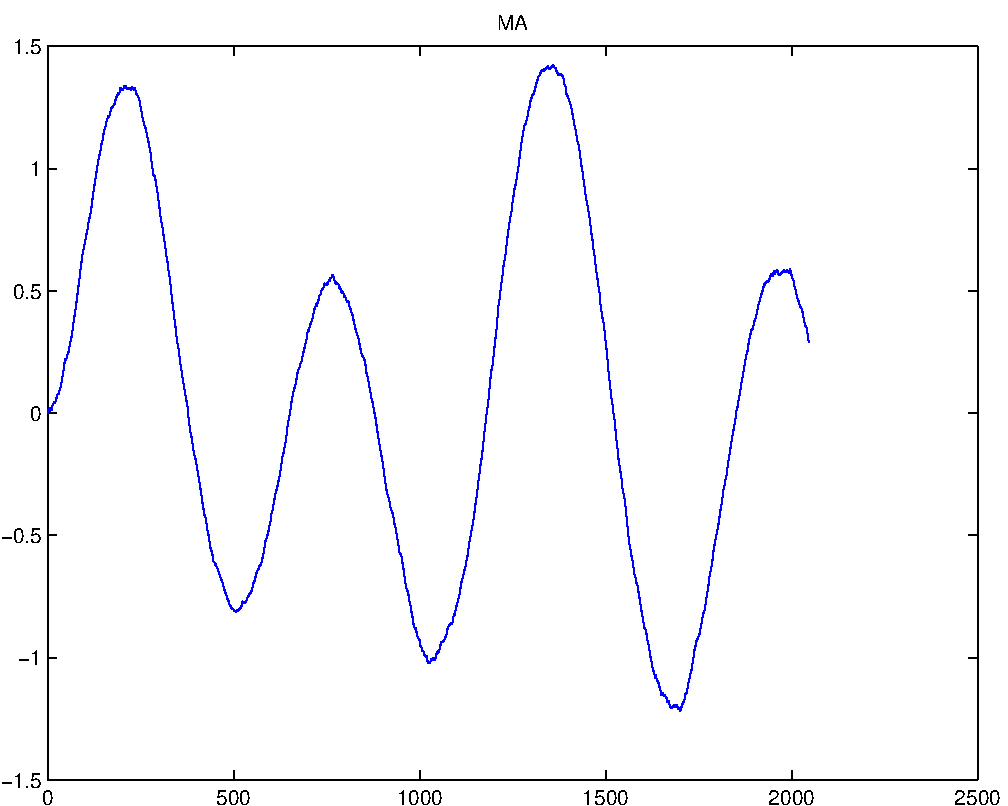
\includegraphics[width=10.0cm,height=10.0cm]{MA.pdf}

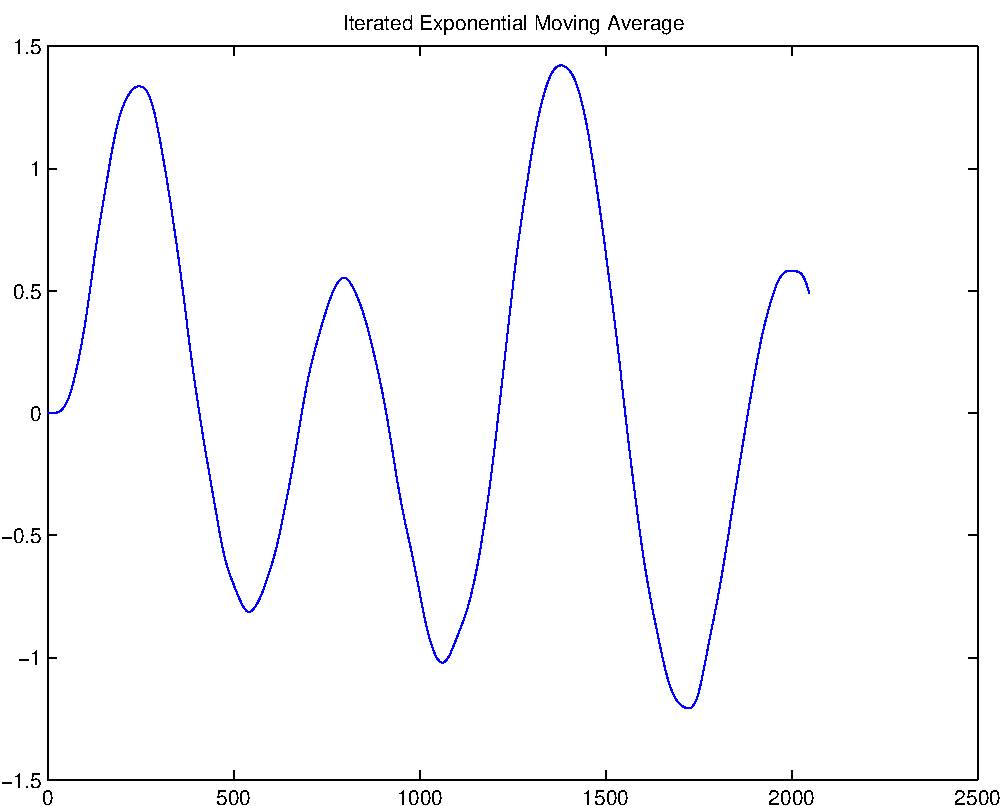
\includegraphics[width=10.0cm,height=10.0cm]{IEMA.pdf}

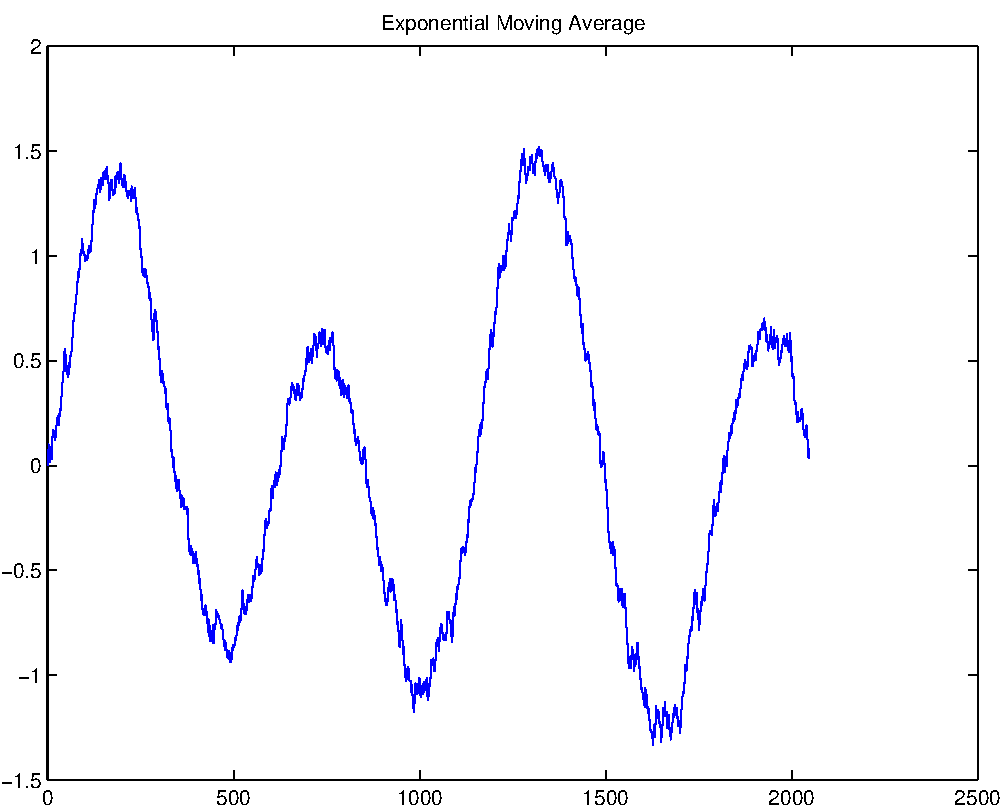
\includegraphics[width=10.0cm,height=10.0cm]{EMA.pdf}

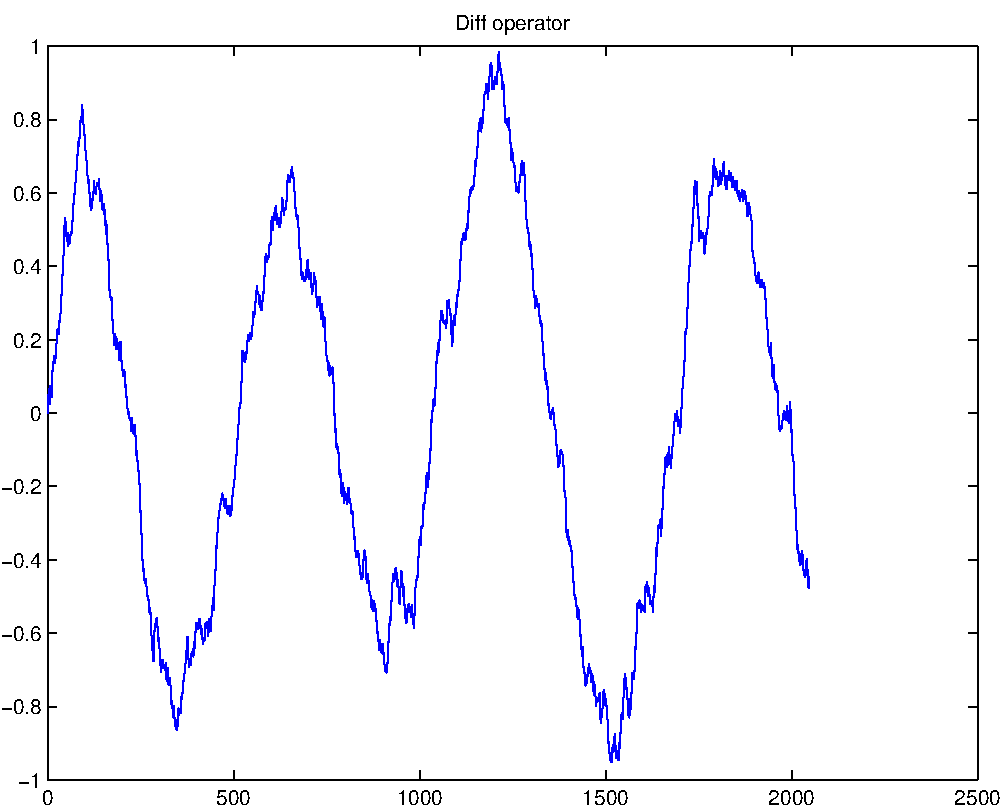
\includegraphics[width=10.0cm,height=10.0cm]{DIFF.pdf}

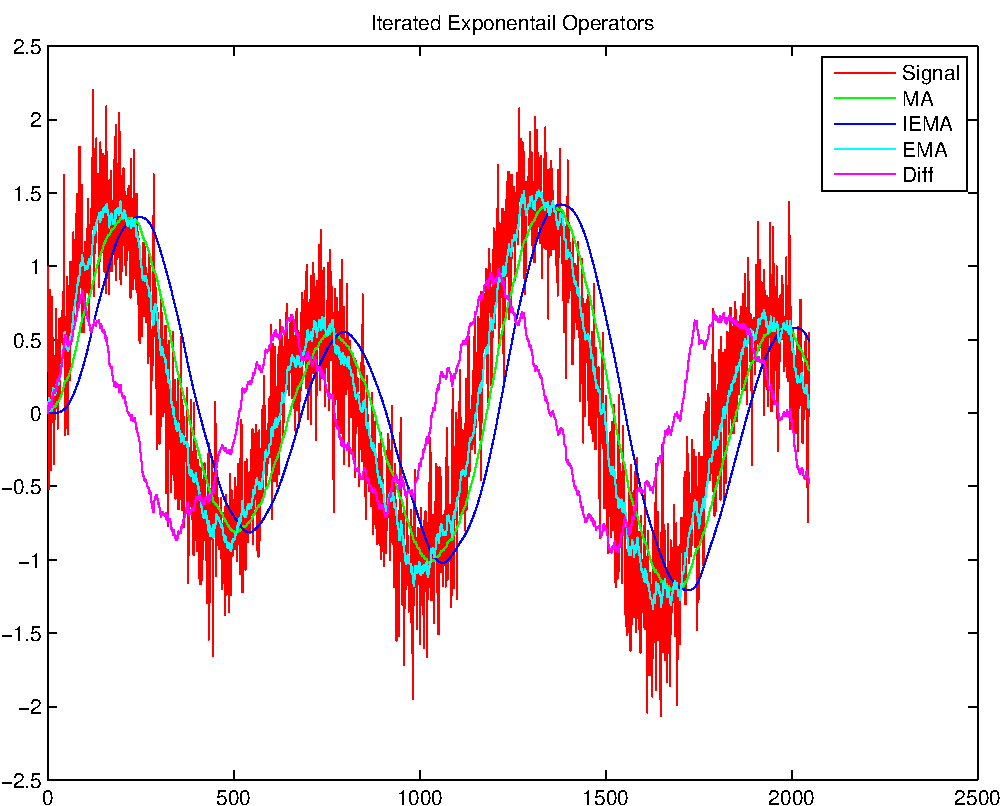
\includegraphics[width=10.0cm,height=10.0cm]{IteratedExponentailOperators.pdf}

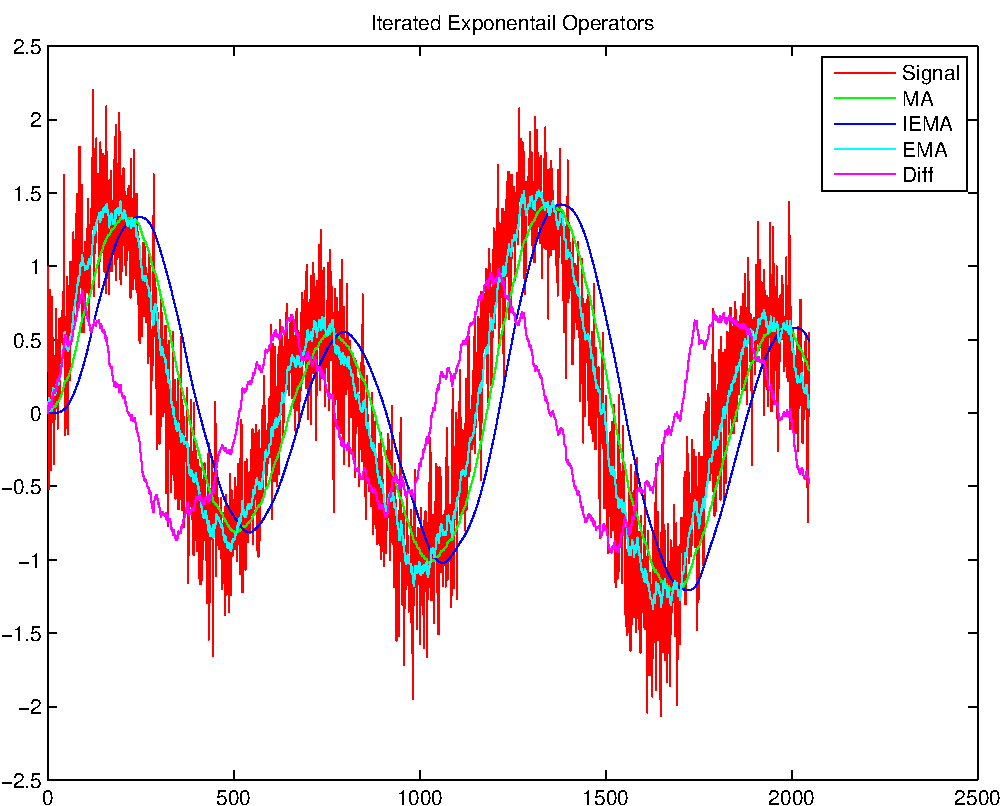
\includegraphics[width=10.0cm,height=10.0cm]{IteratedExponentailOperators.pdf}

QueryPerformanceCounter  =  7.55828
\subsubsection{Testing binary writer}
Binary writer Speedup 1GB Double Matrix 43.0998
Binary reader Speedup 1GB Double Matrix 342.492
Binary writer Speedup 1GB Double vector 45.7839
Binary reader Speedup 1GB Double Matrix 265.353
QueryPerformanceCounter  =  4.48981
\subsubsection{Fast Gauss Transform}
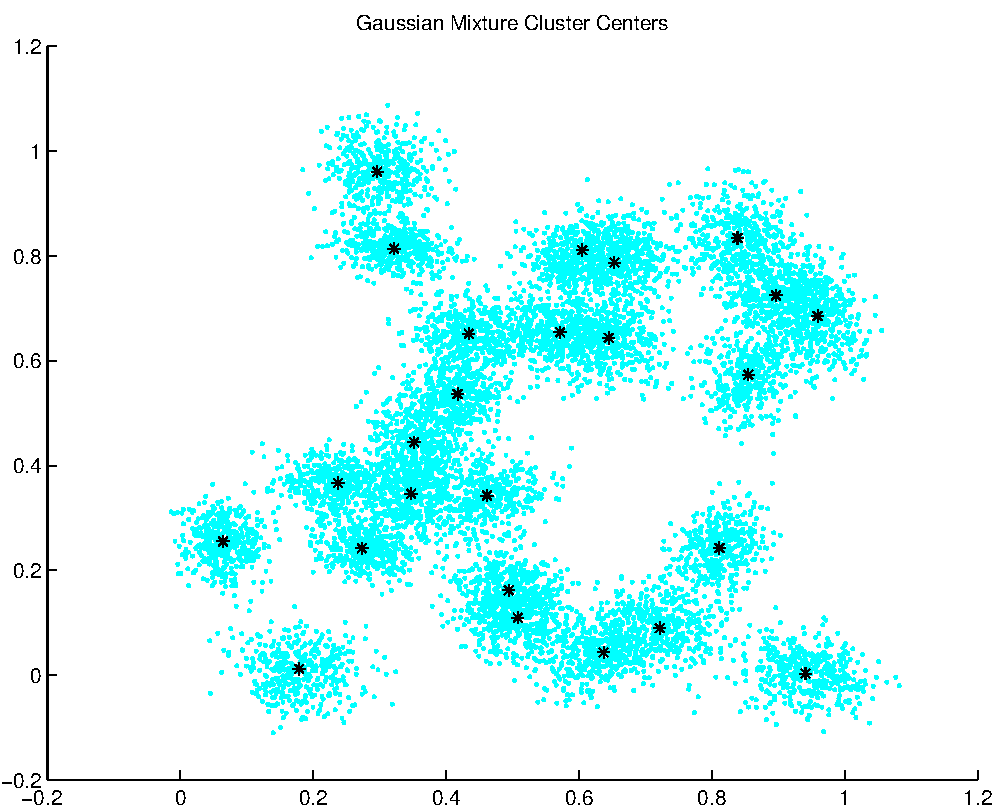
\includegraphics[width=10.0cm,height=10.0cm]{GaussianMixture_ClusterCenters25_Centers.pdf}

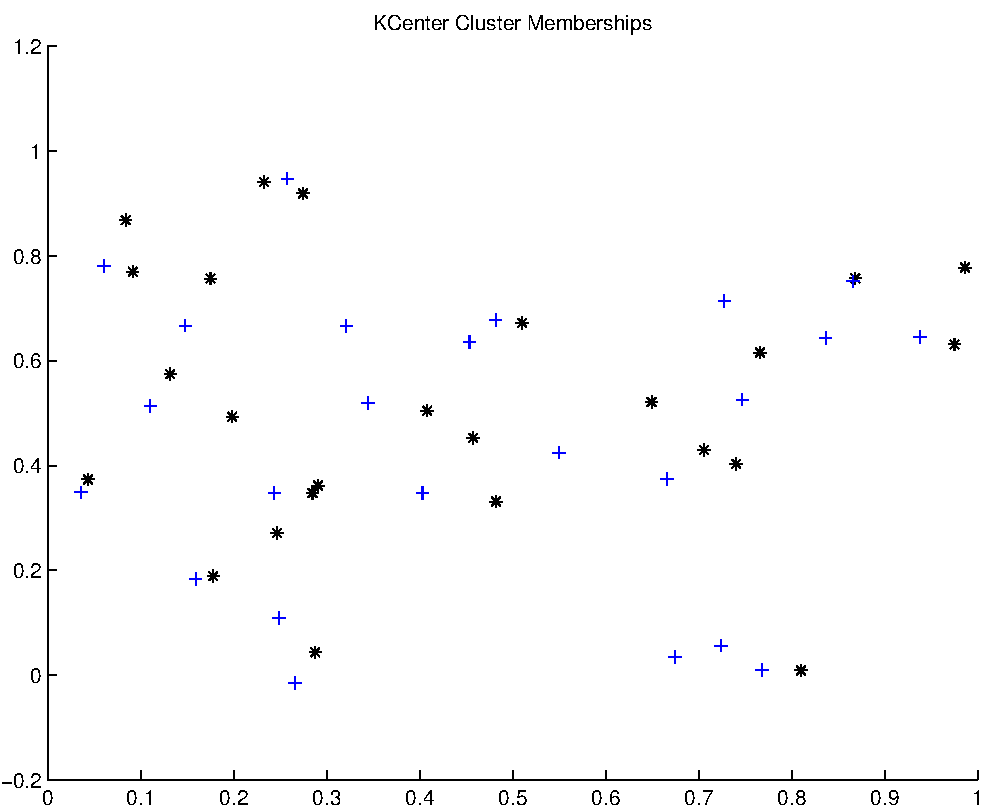
\includegraphics[width=10.0cm,height=10.0cm]{KCenterClusterMemberships_25_Centers.pdf}

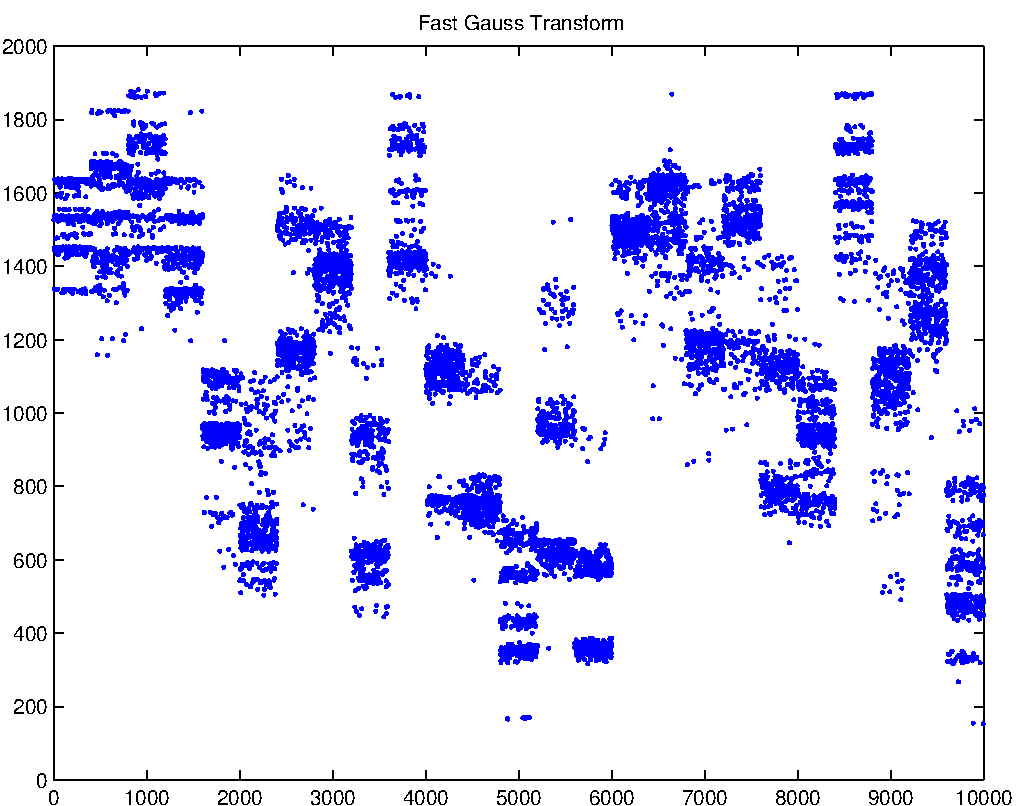
\includegraphics[width=10.0cm,height=10.0cm]{FGT25_Centers.pdf}

QueryPerformanceCounter  =  13.3746
\subsubsection{Testing Gaussian Mixture Point Cloud and Latex Plotting Capabilities.}
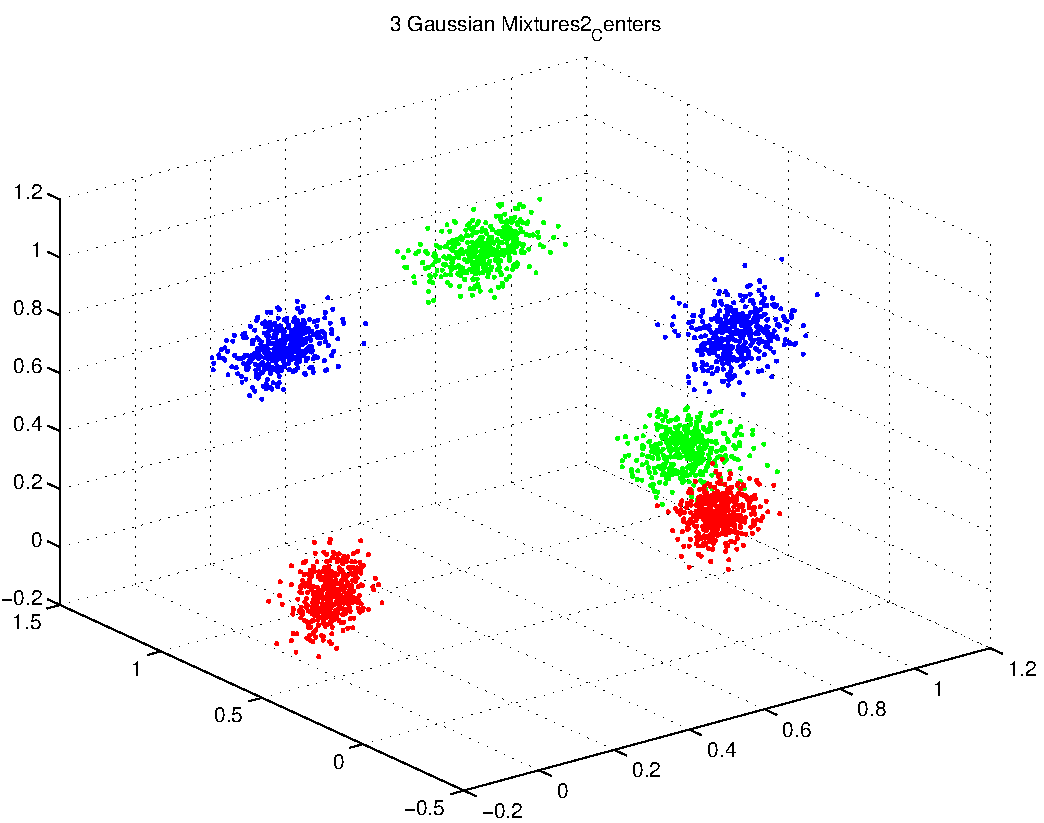
\includegraphics[width=10.0cm,height=10.0cm]{GaussianMixture_Dim_3_Centers2.pdf}

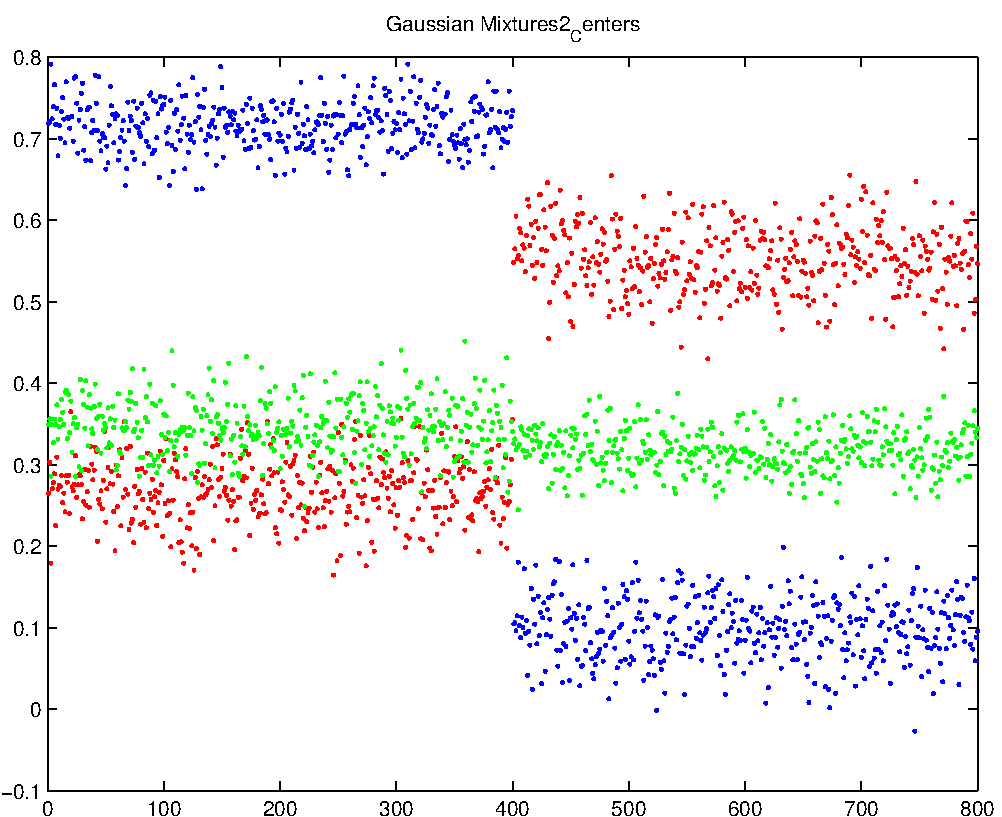
\includegraphics[width=10.0cm,height=10.0cm]{GaussianMixture_Dim_1_Centers2.pdf}

QueryPerformanceCounter  =  3.23435
\subsubsection{Matrix Quick Check <double>}
QueryPerformanceCounter  =  1.40197
\subsubsection{Matrix Quick Check <float>}
QueryPerformanceCounter  =  1.41952
\subsubsection{Intel VSL Function Check}
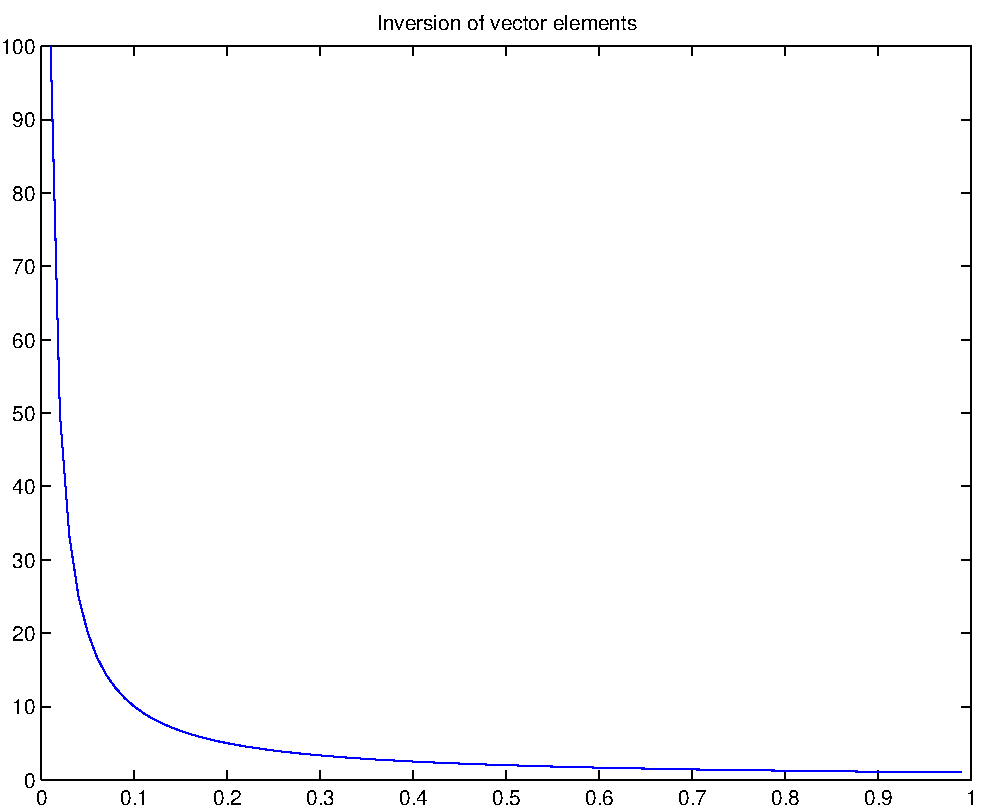
\includegraphics[width=10.0cm,height=10.0cm]{klVSLInv.pdf}

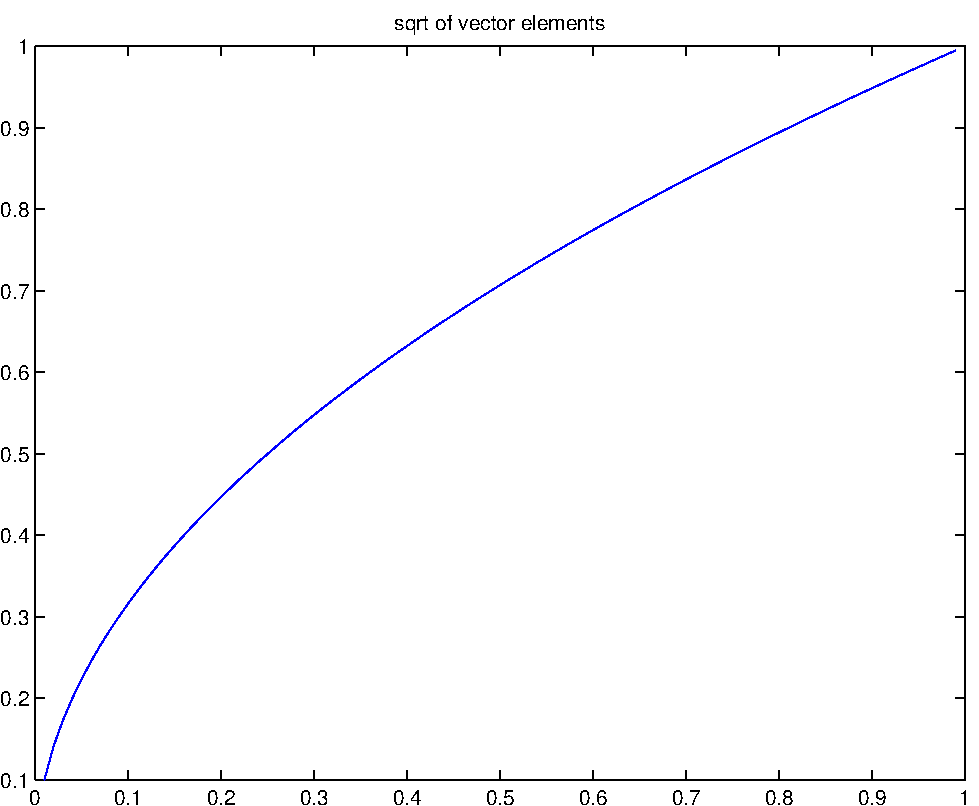
\includegraphics[width=10.0cm,height=10.0cm]{klVSLSqrt.pdf}

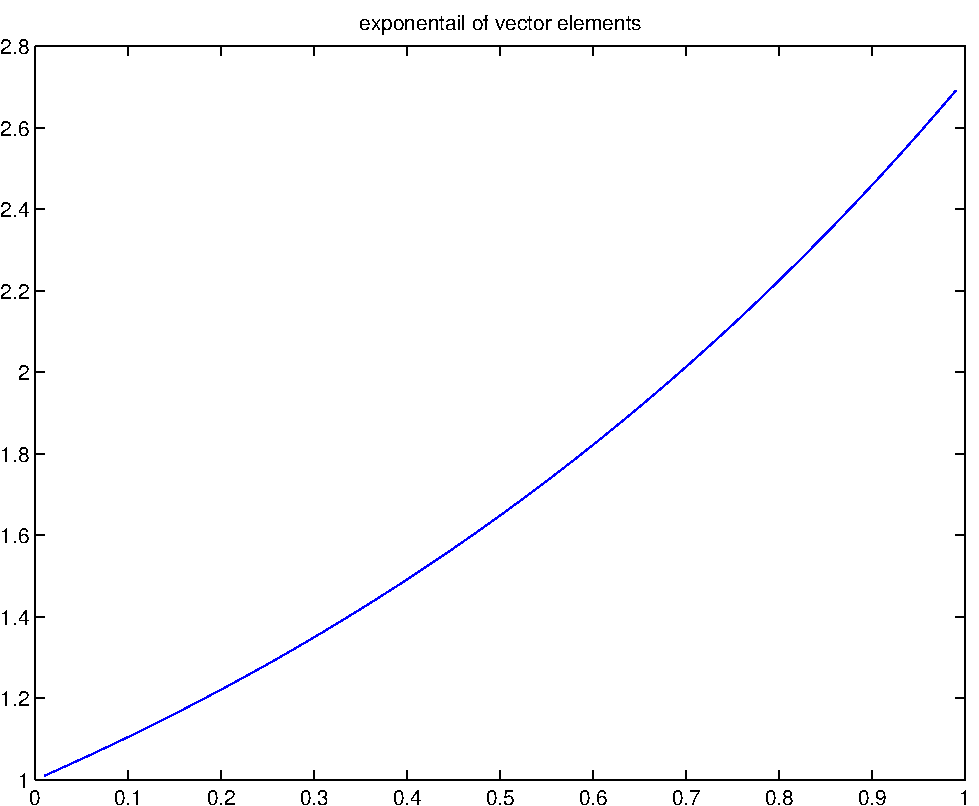
\includegraphics[width=10.0cm,height=10.0cm]{klVSLExp.pdf}

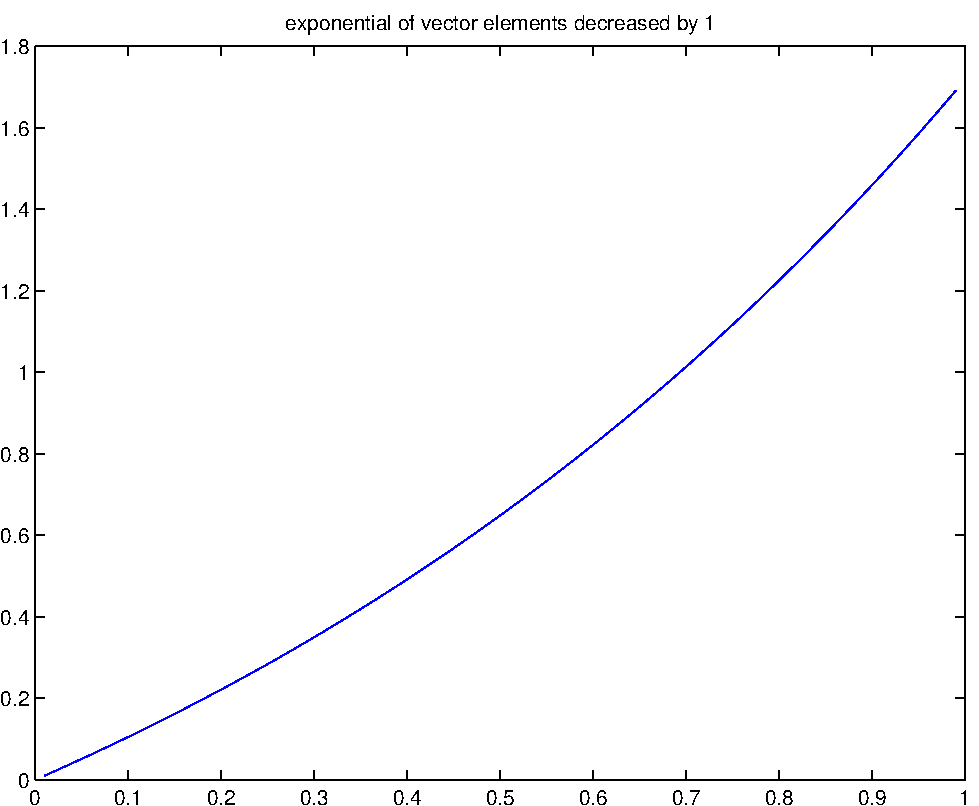
\includegraphics[width=10.0cm,height=10.0cm]{klVSLExpm1.pdf}

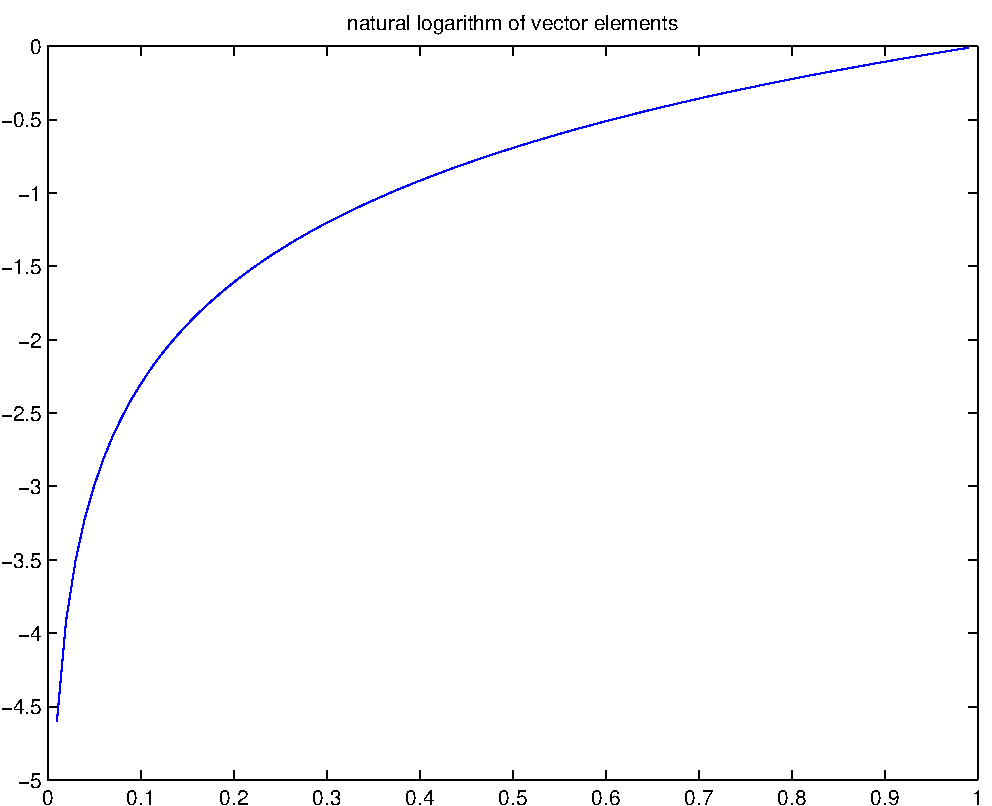
\includegraphics[width=10.0cm,height=10.0cm]{klVSLLn.pdf}

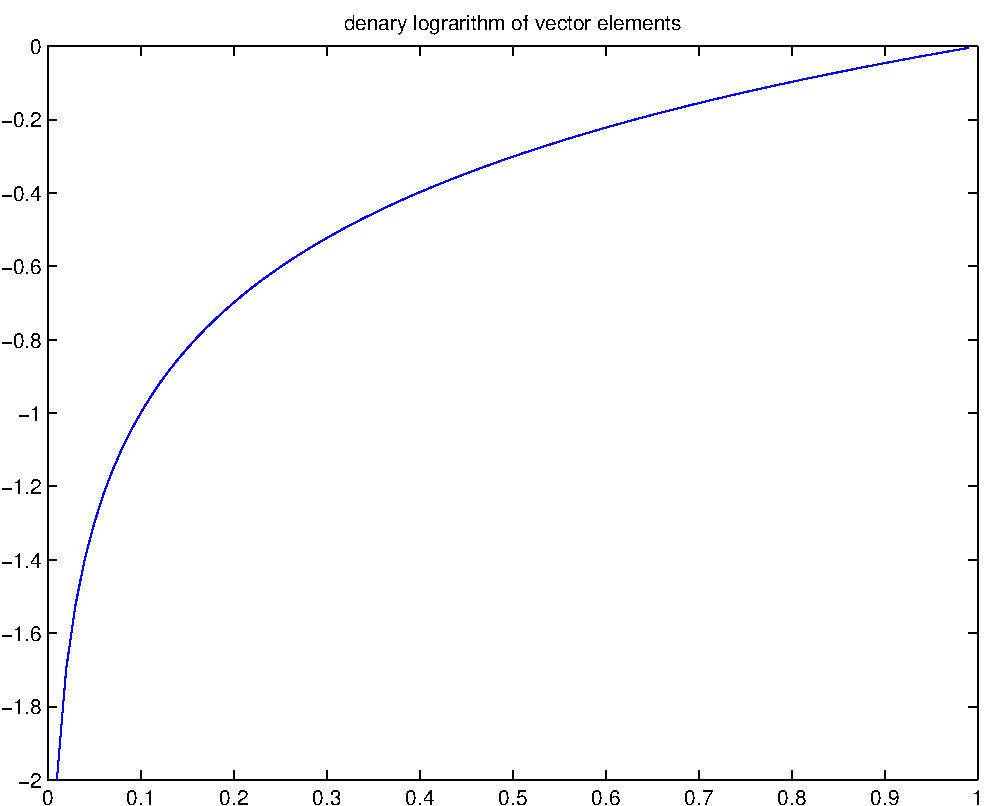
\includegraphics[width=10.0cm,height=10.0cm]{klVSLLog10.pdf}

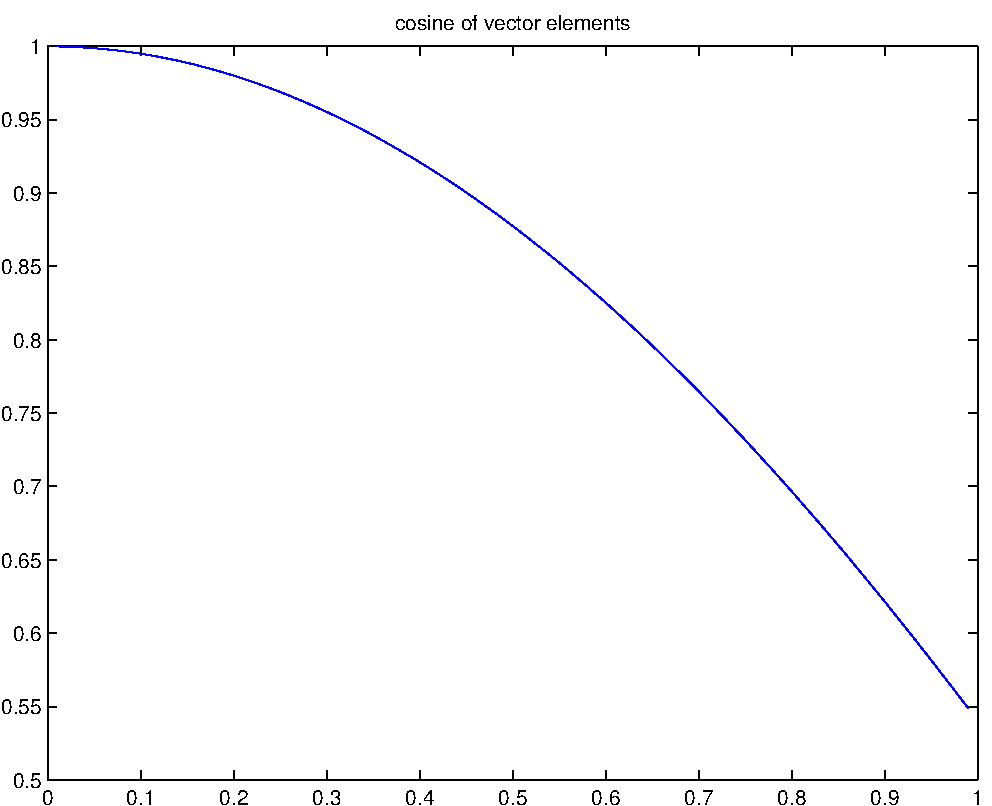
\includegraphics[width=10.0cm,height=10.0cm]{klVSLCos.pdf}

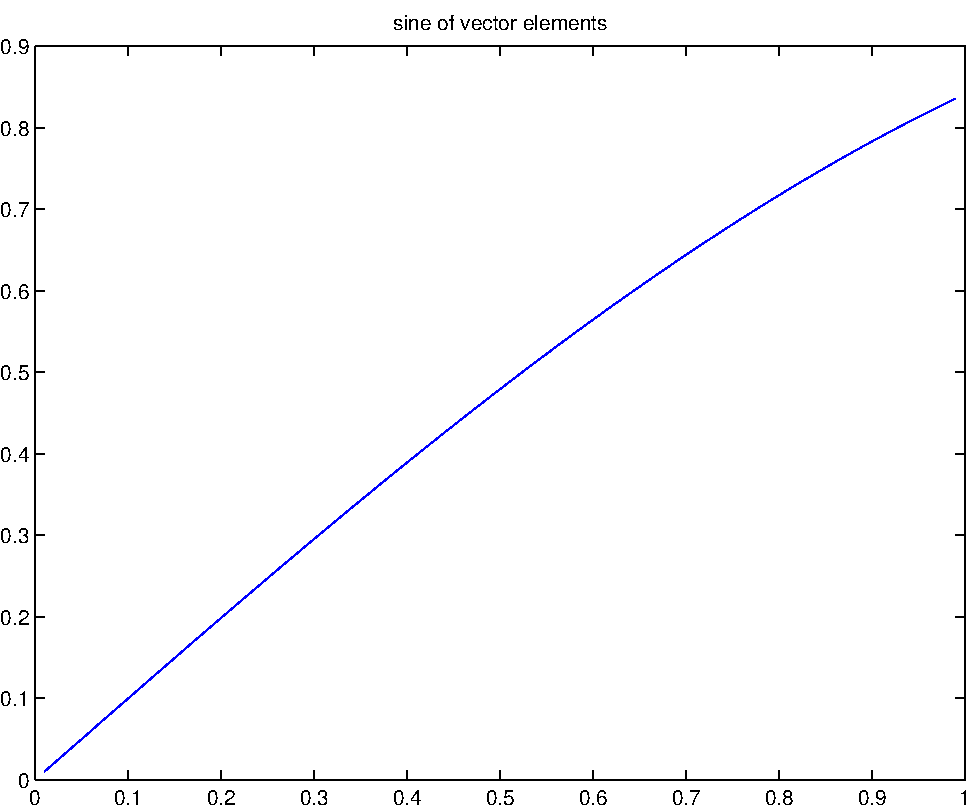
\includegraphics[width=10.0cm,height=10.0cm]{klVSLSin.pdf}

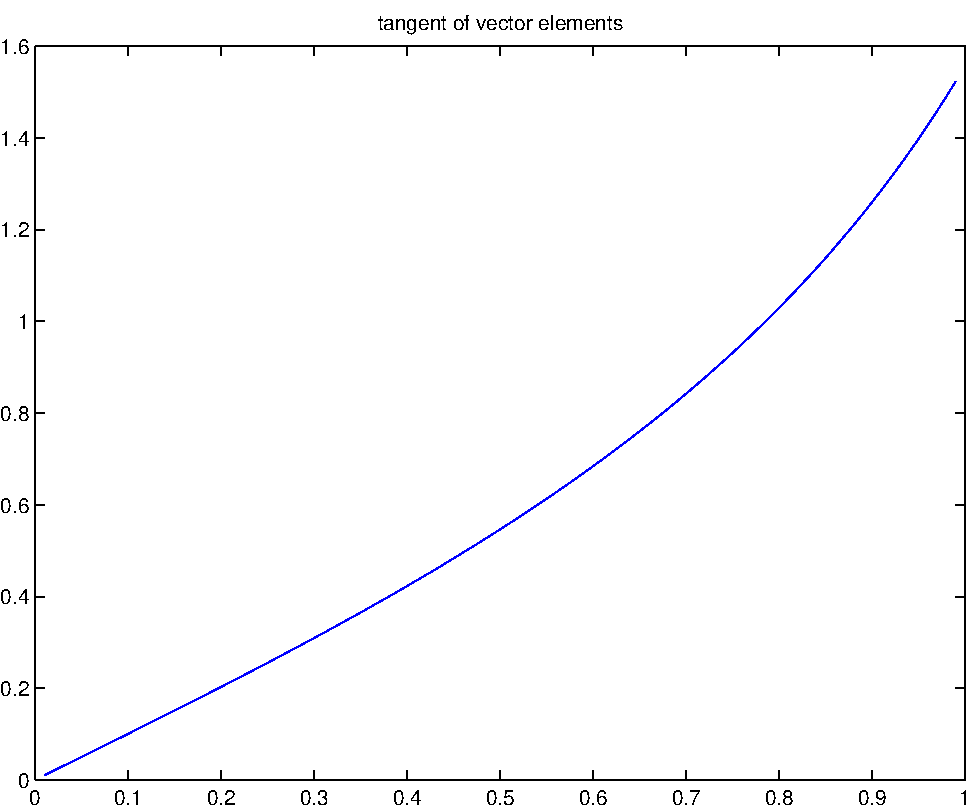
\includegraphics[width=10.0cm,height=10.0cm]{klVSLTan.pdf}

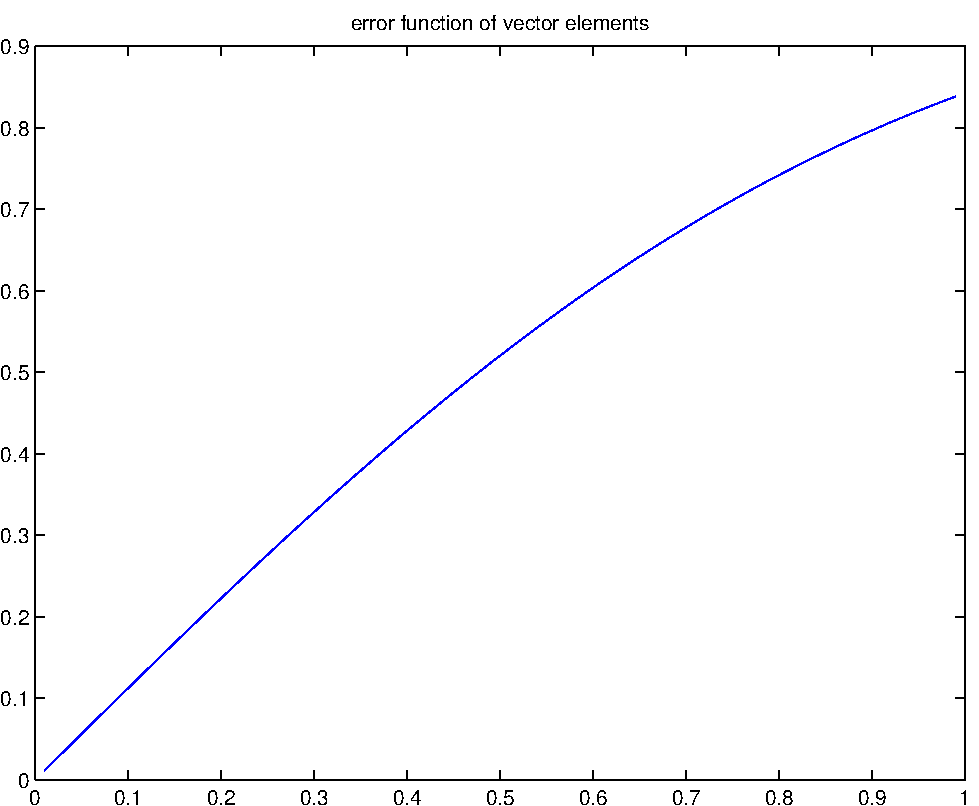
\includegraphics[width=10.0cm,height=10.0cm]{klVSLErf.pdf}

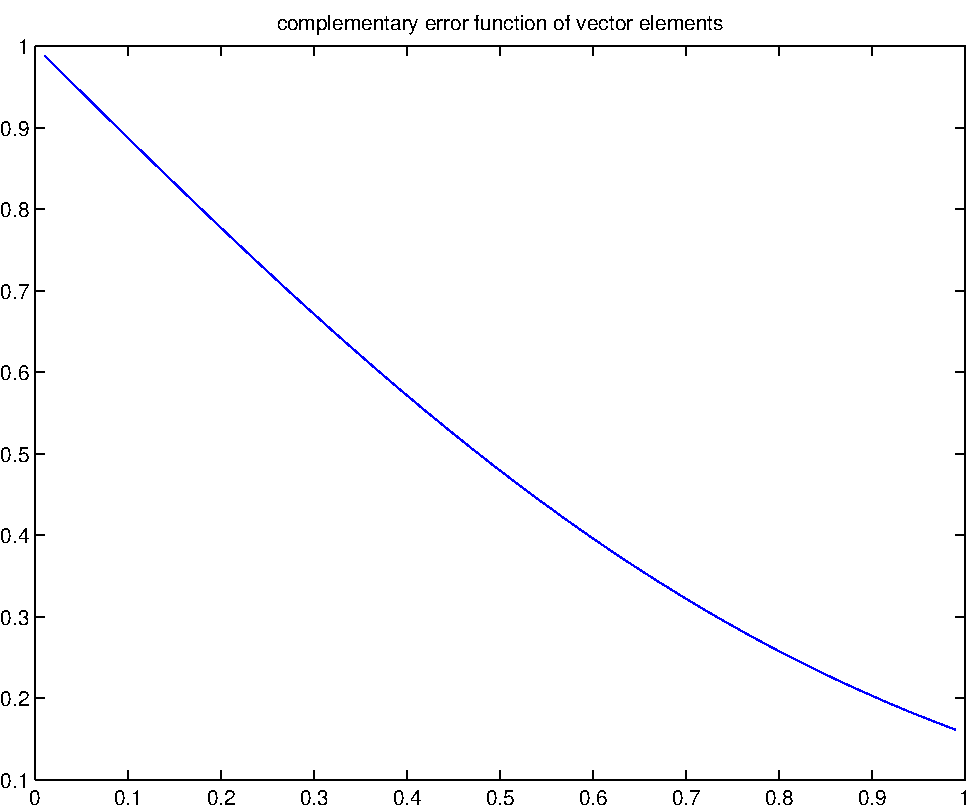
\includegraphics[width=10.0cm,height=10.0cm]{klVSLErfc.pdf}

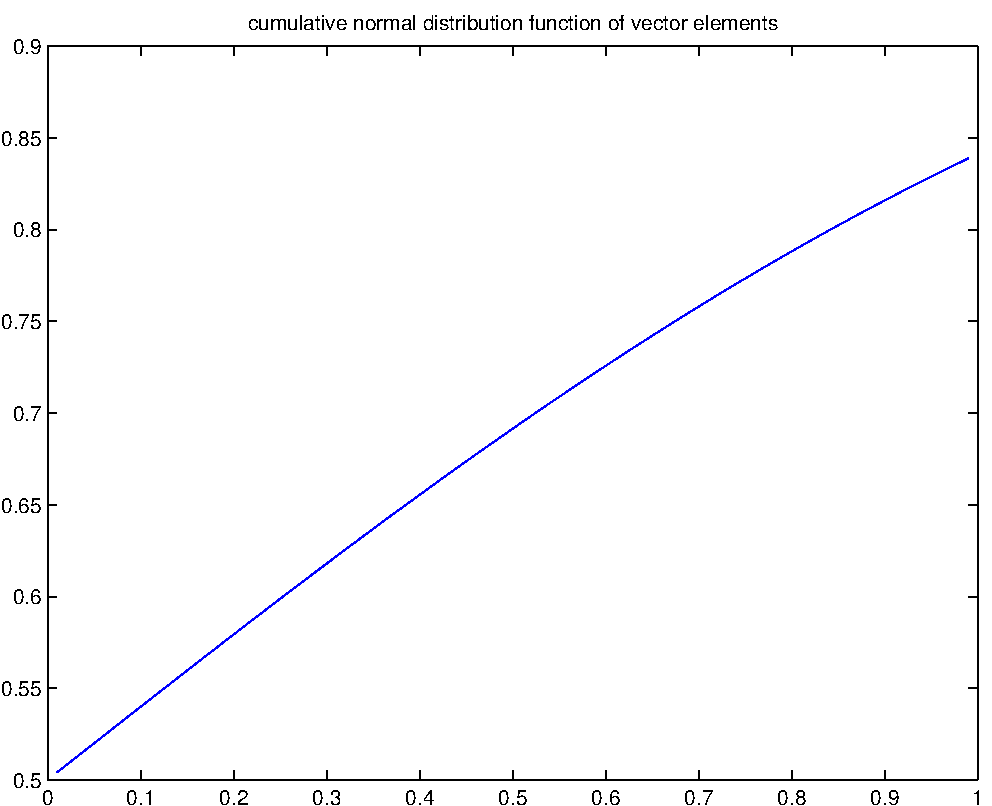
\includegraphics[width=10.0cm,height=10.0cm]{klVSLCdfNorm.pdf}

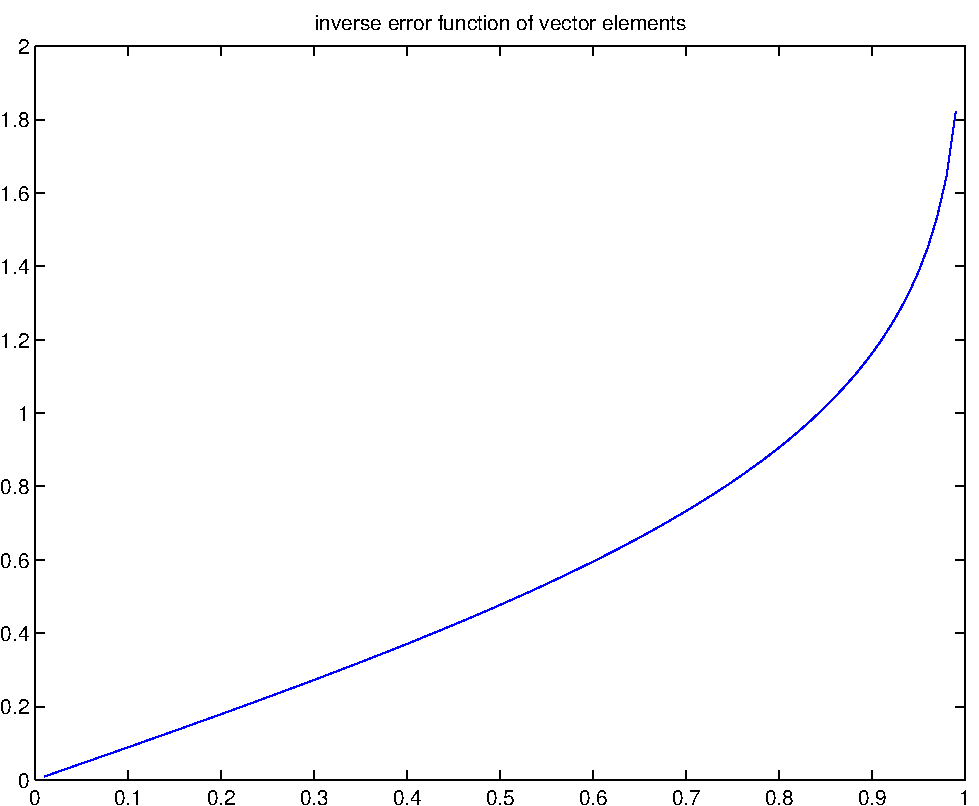
\includegraphics[width=10.0cm,height=10.0cm]{klVSLErfInv.pdf}

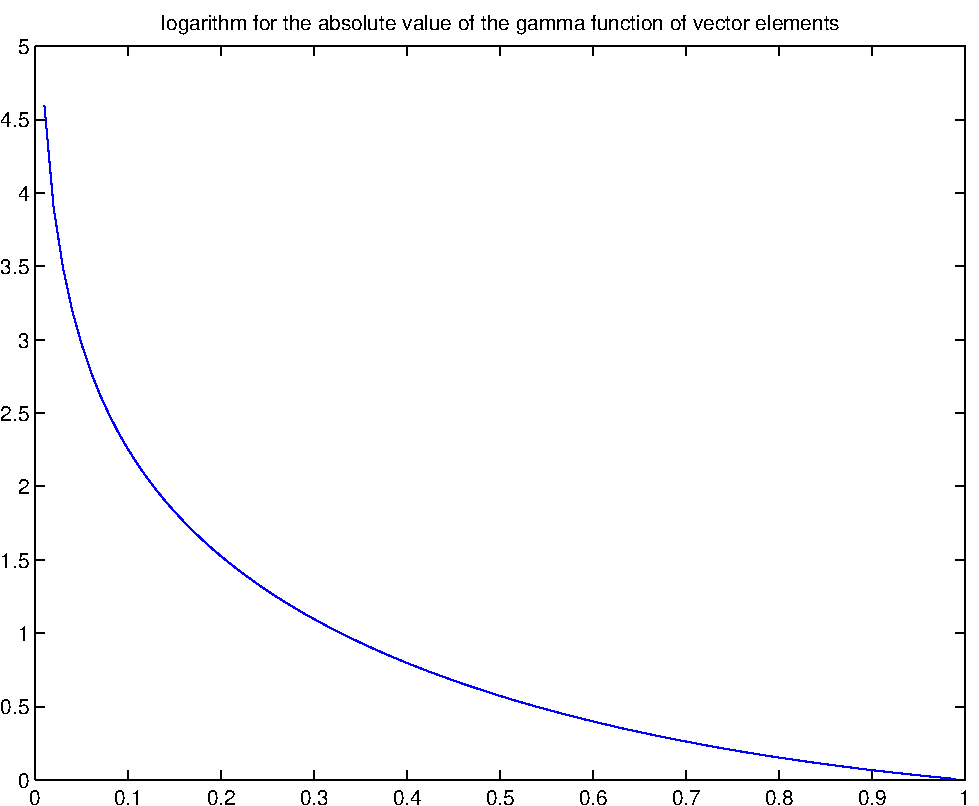
\includegraphics[width=10.0cm,height=10.0cm]{klVSLLGamma.pdf}

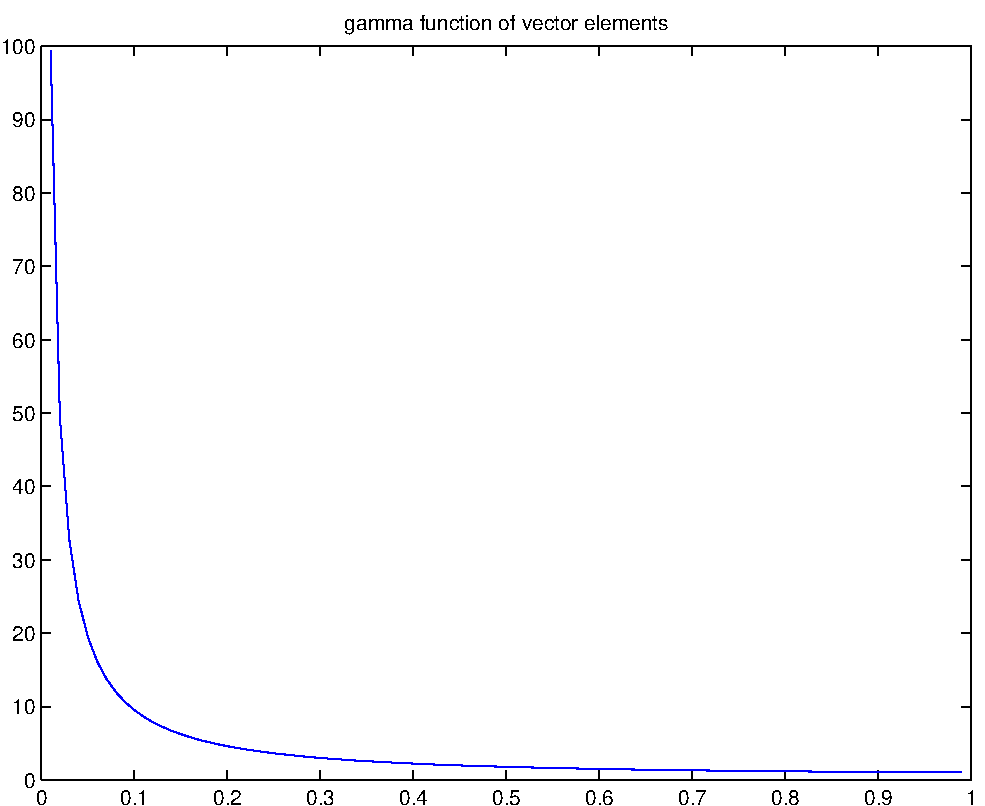
\includegraphics[width=10.0cm,height=10.0cm]{klVSLTGamma.pdf}

QueryPerformanceCounter  =  14.4319
\subsubsection{Gram Matrix Consistency Check}
Sample Size = 4096
Feature dim = 3

$$Sigma$ = \left(
\begin{array}{
ccc}
+1.140 & +1.535 & +0.581 \\
+1.535 & +9.988 & +1.605 \\
+0.581 & +1.605 & +0.428 \\
\end{array}
\right)$ \newline 

$Sample Covariance = \left(
\begin{array}{
ccc}
+1.166 & +1.619 & +0.601 \\
+1.619 & +10.343 & +1.672 \\
+0.601 & +1.672 & +0.443 \\
\end{array}
\right)$ \newline 

$Sample Mean = \left(
\begin{array}{
ccc}
+1.00523 & +1.02214 & +1.00933 \\
\end{array}
\right)$ \newline 

$Sample Covariance-$Omega$ = \left(
\begin{array}{
ccc}
+0.026 & +0.084 & +0.019 \\
+0.084 & +0.355 & +0.067 \\
+0.019 & +0.067 & +0.015 \\
\end{array}
\right)$ \newline 

$Sample Covariance Eigs = \left(
\begin{array}{
ccc}
(+10.91314,+0.00000) & (+0.99837,+0.00000) & (+0.04043,+0.00000) \\
\end{array}
\right)$ \newline 

$Centered Mean = \left(
\begin{array}{
ccc}
-0.00000 & -0.00000 & -0.00000 \\
\end{array}
\right)$ \newline 

$Centered Covariance = \left(
\begin{array}{
ccc}
+1.166 & +1.619 & +0.601 \\
+1.619 & +10.343 & +1.672 \\
+0.601 & +1.672 & +0.443 \\
\end{array}
\right)$ \newline 

$Gram Matrix Gf Not scaled by sample size = \left(
\begin{array}{
ccc}
+4774.238 & +6630.177 & +2460.532 \\
+6630.177 & +42366.044 & +6847.206 \\
+2460.532 & +6847.206 & +1814.850 \\
\end{array}
\right)$ \newline 

$Gram Matrix Gf  scaled by sample size = \left(
\begin{array}{
ccc}
+1.166 & +1.619 & +0.601 \\
+1.619 & +10.343 & +1.672 \\
+0.601 & +1.672 & +0.443 \\
\end{array}
\right)$ \newline 

$SampleCovariance - Scaled Gf = \left(
\begin{array}{
ccc}
+0.000 & +0.000 & +0.000 \\
+0.000 & +0.003 & +0.000 \\
+0.000 & +0.000 & +0.000 \\
\end{array}
\right)$ \newline 

$EigenDecomp of SampleCovariance = \left(
\begin{array}{
ccc}
-0.171 & -0.971 & -0.165 \\
+0.917 & -0.219 & +0.334 \\
-0.360 & -0.094 & +0.928 \\
\end{array}
\right)$ \newline 

$EigenDecomp of Gram Matrix = \left(
\begin{array}{
ccc}
-0.121 & -0.975 & -0.188 \\
-0.332 & +0.219 & -0.918 \\
+0.935 & -0.049 & -0.350 \\
\end{array}
\right)$ \newline 

QueryPerformanceCounter  =  +76.679
\subsubsection{Eigen Solver Checks}
\subsubsection{Haar Distributed Random Orthogonal Matrix $A \in O(n)$}
 Testing Operator Norm
Number of Dimensions: +8

$A = \left(
\begin{array}{
cccccccc}
+0.338 & +0.009 & -0.455 & +0.241 & -0.369 & -0.500 & -0.365 & +0.318 \\
+0.039 & +0.036 & +0.255 & -0.833 & +0.042 & -0.321 & -0.353 & +0.093 \\
-0.011 & +0.056 & +0.156 & -0.140 & -0.844 & -0.055 & +0.295 & -0.389 \\
+0.475 & +0.764 & -0.223 & -0.116 & +0.154 & +0.162 & +0.043 & -0.276 \\
+0.453 & -0.487 & -0.059 & -0.064 & -0.081 & +0.502 & -0.440 & -0.313 \\
+0.188 & -0.204 & +0.161 & +0.203 & +0.326 & -0.603 & +0.061 & -0.619 \\
-0.116 & -0.290 & -0.748 & -0.404 & +0.109 & -0.042 & +0.386 & -0.130 \\
-0.636 & +0.222 & -0.254 & +0.080 & -0.045 & +0.023 & -0.554 & -0.407 \\
\end{array}
\right)$ \newline 

$Det(A) :   A \in O(n)$ = (+1.000,+0.000)

$L = \left(
\begin{array}{
cccccccc}
+1.000 & +0.000 & +0.000 & +0.000 & +0.000 & +0.000 & +0.000 & +0.000 \\
-0.747 & +1.000 & +0.000 & +0.000 & +0.000 & +0.000 & +0.000 & +0.000 \\
+0.182 & -0.356 & +1.000 & +0.000 & +0.000 & +0.000 & +0.000 & +0.000 \\
-0.062 & +0.054 & -0.308 & +1.000 & +0.000 & +0.000 & +0.000 & +0.000 \\
+0.018 & +0.056 & -0.216 & +0.243 & +1.000 & +0.000 & +0.000 & +0.000 \\
-0.531 & +0.137 & +0.628 & -0.590 & +0.553 & +1.000 & +0.000 & +0.000 \\
-0.712 & -0.353 & +0.455 & -0.180 & +0.153 & -0.708 & +1.000 & +0.000 \\
-0.296 & -0.149 & -0.028 & -0.214 & -0.422 & +0.872 & -0.506 & +1.000 \\
\end{array}
\right)$ \newline 

$U = \left(
\begin{array}{
cccccccc}
-0.636 & +0.222 & -0.254 & +0.080 & -0.045 & +0.023 & -0.554 & -0.407 \\
+0.000 & +0.930 & -0.413 & -0.057 & +0.121 & +0.178 & -0.370 & -0.580 \\
+0.000 & +0.000 & -0.849 & -0.438 & +0.160 & +0.017 & +0.355 & -0.262 \\
+0.000 & +0.000 & +0.000 & -0.960 & +0.082 & -0.323 & -0.258 & +0.018 \\
+0.000 & +0.000 & +0.000 & +0.000 & -0.835 & +0.017 & +0.465 & -0.410 \\
+0.000 & +0.000 & +0.000 & +0.000 & +0.000 & -0.724 & -1.241 & +0.583 \\
+0.000 & +0.000 & +0.000 & +0.000 & +0.000 & +0.000 & -2.123 & -0.210 \\
+0.000 & +0.000 & +0.000 & +0.000 & +0.000 & +0.000 & +0.000 & -1.616 \\
\end{array}
\right)$ \newline 

$L * U  = \left(
\begin{array}{
cccccccc}
-0.636 & +0.222 & -0.254 & +0.080 & -0.045 & +0.023 & -0.554 & -0.407 \\
+0.475 & +0.764 & -0.223 & -0.116 & +0.154 & +0.162 & +0.043 & -0.276 \\
-0.116 & -0.290 & -0.748 & -0.404 & +0.109 & -0.042 & +0.386 & -0.130 \\
+0.039 & +0.036 & +0.255 & -0.833 & +0.042 & -0.321 & -0.353 & +0.093 \\
-0.011 & +0.056 & +0.156 & -0.140 & -0.844 & -0.055 & +0.295 & -0.389 \\
+0.338 & +0.009 & -0.455 & +0.241 & -0.369 & -0.500 & -0.365 & +0.318 \\
+0.453 & -0.487 & -0.059 & -0.064 & -0.081 & +0.502 & -0.440 & -0.313 \\
+0.188 & -0.204 & +0.161 & +0.203 & +0.326 & -0.603 & +0.061 & -0.619 \\
\end{array}
\right)$ \newline 

$Det(L) :    = (+1.000,+0.000)     Det(U) :    = (-1.000,+0.000)     Det(LU) :    = (-1.000,-0.000)$

$||A||_{L_1}$  = +2.544

$||A||_{L_{\infty}}$ = +2.595

$||A^{-1}||_{L_1}$  = +2.595

$||A^{-1}||_{L_{\infty}}$ = +2.544

$||A||_{L_{\infty}} * ||A^{-1}||_{L_{\infty}} = +6.602$

$||A||_{L_1} * ||A^{-1}||_{L_1} = +6.602$

Frobenious Norm  $||A||_{\textit{F}}$ via $\sum\limits_{i,j =0}^{n} \|A_{i,j}|$   of  $A \in O(n)$  +2.828

$L_1$ condition number of Haar Distributed Random Orthogonal Matrix $A \in O(n)$ +5.630

$A = \left(
\begin{array}{
cccccccc}
+0.338 & +0.009 & -0.455 & +0.241 & -0.369 & -0.500 & -0.365 & +0.318 \\
+0.039 & +0.036 & +0.255 & -0.833 & +0.042 & -0.321 & -0.353 & +0.093 \\
-0.011 & +0.056 & +0.156 & -0.140 & -0.844 & -0.055 & +0.295 & -0.389 \\
+0.475 & +0.764 & -0.223 & -0.116 & +0.154 & +0.162 & +0.043 & -0.276 \\
+0.453 & -0.487 & -0.059 & -0.064 & -0.081 & +0.502 & -0.440 & -0.313 \\
+0.188 & -0.204 & +0.161 & +0.203 & +0.326 & -0.603 & +0.061 & -0.619 \\
-0.116 & -0.290 & -0.748 & -0.404 & +0.109 & -0.042 & +0.386 & -0.130 \\
-0.636 & +0.222 & -0.254 & +0.080 & -0.045 & +0.023 & -0.554 & -0.407 \\
\end{array}
\right)$ \newline 

$L_{\infty}$ condition number of Haar Distributed Random Orthogonal Matrix $A \in O(n)$ +5.369

Eigenvalues of $A \in O(n)$

(+0.269,+0.963), (+0.269,-0.963), (-0.292,+0.956), (-0.292,-0.956), (-0.991,+0.137), (-0.991,-0.137), (+0.867,+0.497), (+0.867,-0.497)

 $|\lambda | : \lambda \in \sigma(A) , A \in O(n)$

+1.000, +1.000, +1.000, +1.000, +1.000, +1.000, +1.000, +1.000


Calculating $A^{\dag} A,$  we expect $A^{\dag} A \approx I$

$A^{\dag} A = \left(
\begin{array}{
cccccccc}
+1.000 & -0.000 & +0.000 & -0.000 & +0.000 & +0.000 & +0.000 & -0.000 \\
-0.000 & +1.000 & -0.000 & -0.000 & +0.000 & -0.000 & -0.000 & +0.000 \\
+0.000 & -0.000 & +1.000 & +0.000 & -0.000 & -0.000 & -0.000 & -0.000 \\
-0.000 & -0.000 & +0.000 & +1.000 & -0.000 & +0.000 & -0.000 & +0.000 \\
+0.000 & +0.000 & -0.000 & -0.000 & +1.000 & -0.000 & -0.000 & +0.000 \\
+0.000 & -0.000 & -0.000 & +0.000 & -0.000 & +1.000 & +0.000 & +0.000 \\
+0.000 & -0.000 & -0.000 & -0.000 & -0.000 & +0.000 & +1.000 & +0.000 \\
-0.000 & +0.000 & -0.000 & +0.000 & +0.000 & +0.000 & +0.000 & +1.000 \\
\end{array}
\right)$ \newline 

Calculating $A^{-1} ,  A \in O(n)$.

$A^{-1} = \left(
\begin{array}{
cccccccc}
+0.338 & +0.039 & -0.011 & +0.475 & +0.453 & +0.188 & -0.116 & -0.636 \\
+0.009 & +0.036 & +0.056 & +0.764 & -0.487 & -0.204 & -0.290 & +0.222 \\
-0.455 & +0.255 & +0.156 & -0.223 & -0.059 & +0.161 & -0.748 & -0.254 \\
+0.241 & -0.833 & -0.140 & -0.116 & -0.064 & +0.203 & -0.404 & +0.080 \\
-0.369 & +0.042 & -0.844 & +0.154 & -0.081 & +0.326 & +0.109 & -0.045 \\
-0.500 & -0.321 & -0.055 & +0.162 & +0.502 & -0.603 & -0.042 & +0.023 \\
-0.365 & -0.353 & +0.295 & +0.043 & -0.440 & +0.061 & +0.386 & -0.554 \\
+0.318 & +0.093 & -0.389 & -0.276 & -0.313 & -0.619 & -0.130 & -0.407 \\
\end{array}
\right)$ \newline 

Calculating $A^{-1} *A  ,  A \in O(n)$.   We expect $A^{-1} *A  \approx I$. 

$A^{-1} *A = \left(
\begin{array}{
cccccccc}
+1.000 & +0.000 & +0.000 & +0.000 & +0.000 & -0.000 & +0.000 & +0.000 \\
-0.000 & +1.000 & +0.000 & +0.000 & -0.000 & +0.000 & -0.000 & -0.000 \\
-0.000 & -0.000 & +1.000 & -0.000 & +0.000 & -0.000 & +0.000 & -0.000 \\
-0.000 & -0.000 & -0.000 & +1.000 & +0.000 & -0.000 & +0.000 & +0.000 \\
-0.000 & -0.000 & +0.000 & -0.000 & +1.000 & -0.000 & +0.000 & +0.000 \\
+0.000 & +0.000 & +0.000 & +0.000 & -0.000 & +1.000 & -0.000 & -0.000 \\
+0.000 & +0.000 & -0.000 & -0.000 & -0.000 & -0.000 & +1.000 & +0.000 \\
+0.000 & -0.000 & +0.000 & -0.000 & +0.000 & +0.000 & -0.000 & +1.000 \\
\end{array}
\right)$ \newline 

Calculating SVD of  $A \in O(n)$

$U = \left(
\begin{array}{
cccccccc}
+0.434 & -0.706 & -0.108 & +0.001 & +0.279 & +0.353 & -0.308 & -0.068 \\
-0.107 & -0.385 & +0.335 & +0.487 & -0.636 & +0.176 & +0.233 & +0.040 \\
-0.047 & -0.071 & +0.208 & +0.436 & +0.257 & -0.494 & -0.165 & -0.650 \\
-0.403 & -0.345 & -0.495 & +0.246 & +0.344 & -0.168 & +0.468 & +0.218 \\
-0.284 & +0.277 & +0.079 & +0.539 & +0.280 & +0.356 & -0.475 & +0.339 \\
+0.201 & -0.150 & +0.607 & -0.052 & +0.302 & -0.396 & +0.110 & +0.553 \\
-0.633 & -0.360 & +0.083 & -0.400 & -0.166 & -0.197 & -0.483 & +0.049 \\
-0.338 & -0.009 & +0.455 & -0.241 & +0.369 & +0.500 & +0.365 & -0.318 \\
\end{array}
\right)$ \newline 

$S = \left(
\begin{array}{
cccccccc}
+1.000 & +0.000 & +0.000 & +0.000 & +0.000 & +0.000 & +0.000 & +0.000 \\
+0.000 & +1.000 & +0.000 & +0.000 & +0.000 & +0.000 & +0.000 & +0.000 \\
+0.000 & +0.000 & +1.000 & +0.000 & +0.000 & +0.000 & +0.000 & +0.000 \\
+0.000 & +0.000 & +0.000 & +1.000 & +0.000 & +0.000 & +0.000 & +0.000 \\
+0.000 & +0.000 & +0.000 & +0.000 & +1.000 & +0.000 & +0.000 & +0.000 \\
+0.000 & +0.000 & +0.000 & +0.000 & +0.000 & +1.000 & +0.000 & +0.000 \\
+0.000 & +0.000 & +0.000 & +0.000 & +0.000 & +0.000 & +1.000 & +0.000 \\
+0.000 & +0.000 & +0.000 & +0.000 & +0.000 & +0.000 & +0.000 & +1.000 \\
\end{array}
\right)$ \newline 

$V = \left(
\begin{array}{
cccccccc}
+0.000 & +0.000 & -0.000 & +0.000 & +0.000 & -0.000 & +0.000 & -1.000 \\
-0.036 & -0.500 & -0.148 & -0.436 & -0.333 & +0.353 & +0.548 & -0.000 \\
-0.380 & +0.543 & -0.018 & -0.354 & -0.573 & -0.324 & +0.046 & +0.000 \\
-0.204 & -0.547 & -0.042 & -0.387 & -0.017 & -0.314 & -0.639 & +0.000 \\
+0.858 & +0.113 & -0.020 & -0.387 & -0.044 & -0.314 & +0.022 & +0.000 \\
+0.110 & -0.112 & +0.901 & +0.072 & -0.350 & +0.157 & -0.109 & +0.000 \\
+0.141 & -0.315 & -0.236 & +0.615 & -0.536 & -0.393 & +0.074 & +0.000 \\
-0.212 & -0.176 & +0.329 & -0.042 & +0.386 & -0.628 & +0.520 & +0.000 \\
\end{array}
\right)$ \newline 

$U S V = \left(
\begin{array}{
cccccccc}
+0.315 & +0.395 & +0.469 & +0.077 & +0.300 & -0.083 & -0.483 & -0.434 \\
-0.714 & -0.064 & +0.160 & +0.261 & -0.215 & -0.286 & -0.502 & +0.107 \\
+0.115 & +0.161 & -0.636 & -0.420 & -0.104 & +0.085 & -0.599 & +0.047 \\
+0.447 & -0.359 & -0.147 & +0.364 & +0.271 & -0.494 & -0.195 & +0.403 \\
-0.009 & -0.309 & +0.474 & -0.747 & +0.102 & -0.155 & -0.081 & +0.284 \\
-0.101 & +0.380 & -0.193 & -0.230 & -0.017 & -0.781 & +0.325 & -0.201 \\
-0.180 & +0.592 & +0.025 & +0.034 & +0.433 & +0.152 & +0.070 & +0.633 \\
+0.367 & +0.310 & +0.256 & +0.067 & -0.763 & -0.056 & -0.015 & +0.338 \\
\end{array}
\right)$ \newline 

Calculating first few eigenvectors of $A \in O(n)$ using LAPACK syevx

\subsubsection{Wishart Matrix $A \in W(n)$}
$L_1$ condition number of Wishart Matrix +1489.694
$L_infty$ condition number of Wishart Matrix +1489.694
\subsubsection{Gaussian Orthogonal Ensemble $A \in GOE(n)$}
$L_1$ condition number of GOE Matrix +66.900
$L_\infty$ condition number of GOE Matrix +66.900
\subsubsection{The Identity Matrix $I \in M(n)$}
$L_1$ condition number of $I$ = +1.000
$L_\infty$ condition number of $I$ = +1.000
QueryPerformanceCounter  =  +2.127
\subsubsection{Generate Tracey Widom Sample}
\subsubsection{Sample from $W_n m$ times and calculate empirical PDF of the first eig}
Here we generate histograms of $\lambda_1$ for GOE (Gaussian Orthogonal Ensemble), and W (Wishart) 		 distributed of random matrices
These should approximate the celebrated Tracy Widom distribution.
Dimension $n = +128$

Sample size $m = 32$

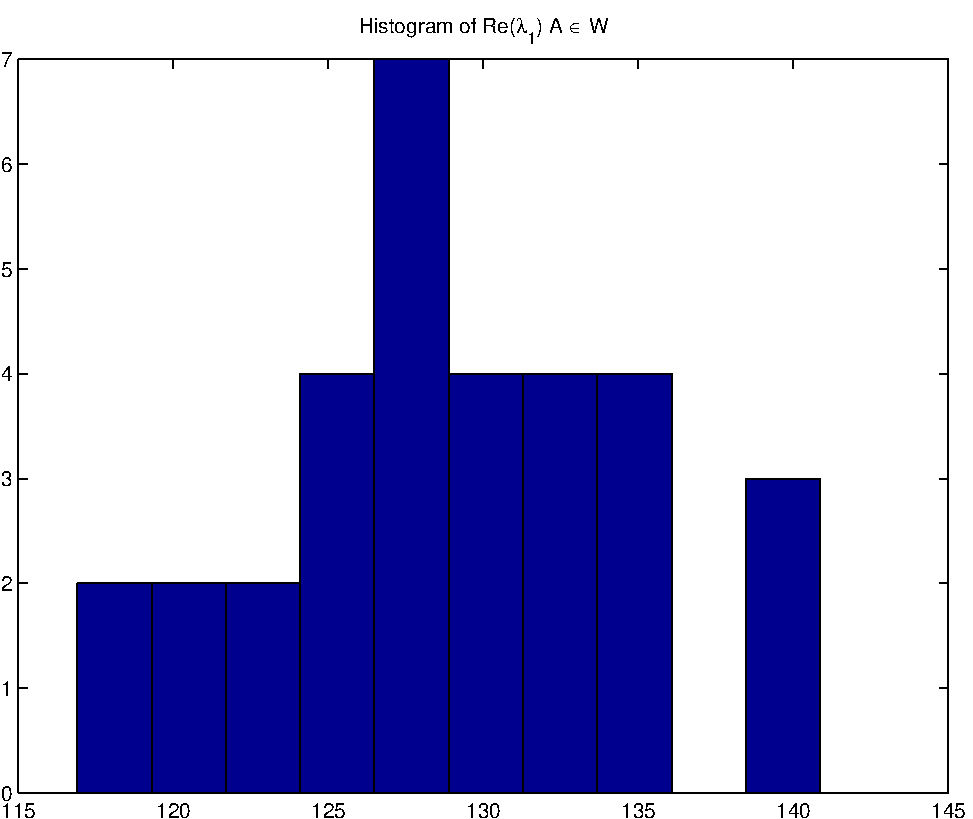
\includegraphics[width=10.0cm,height=10.0cm]{Re_TraceyWidom.pdf}

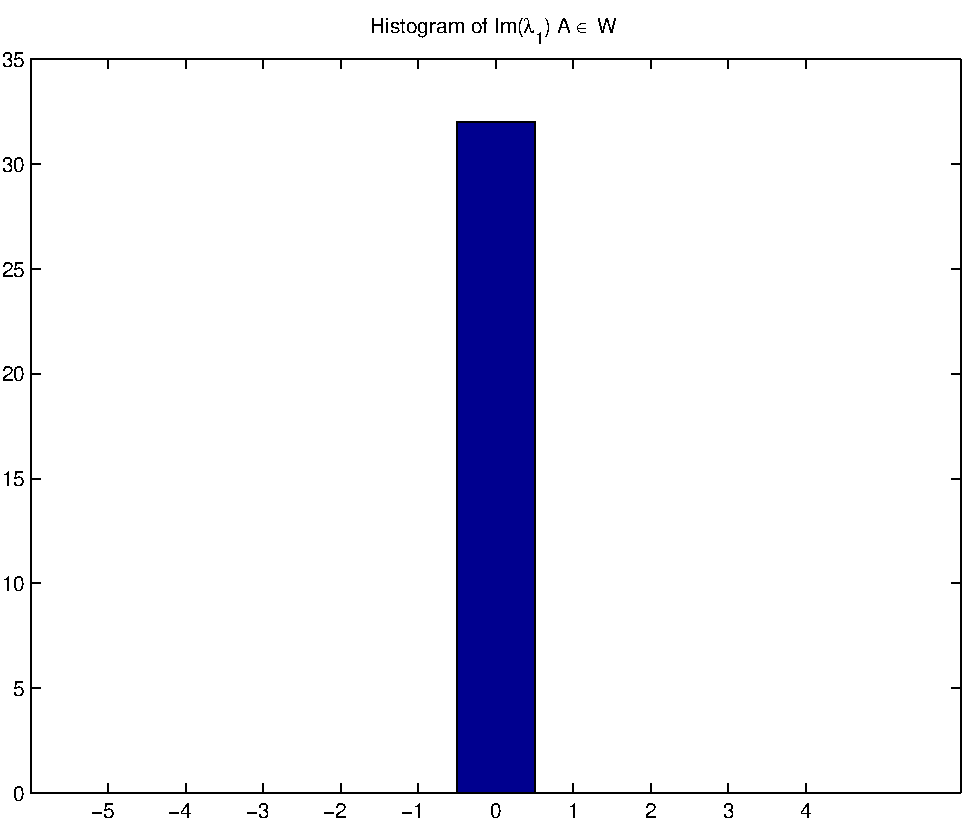
\includegraphics[width=10.0cm,height=10.0cm]{Im_TraceyWidom.pdf}

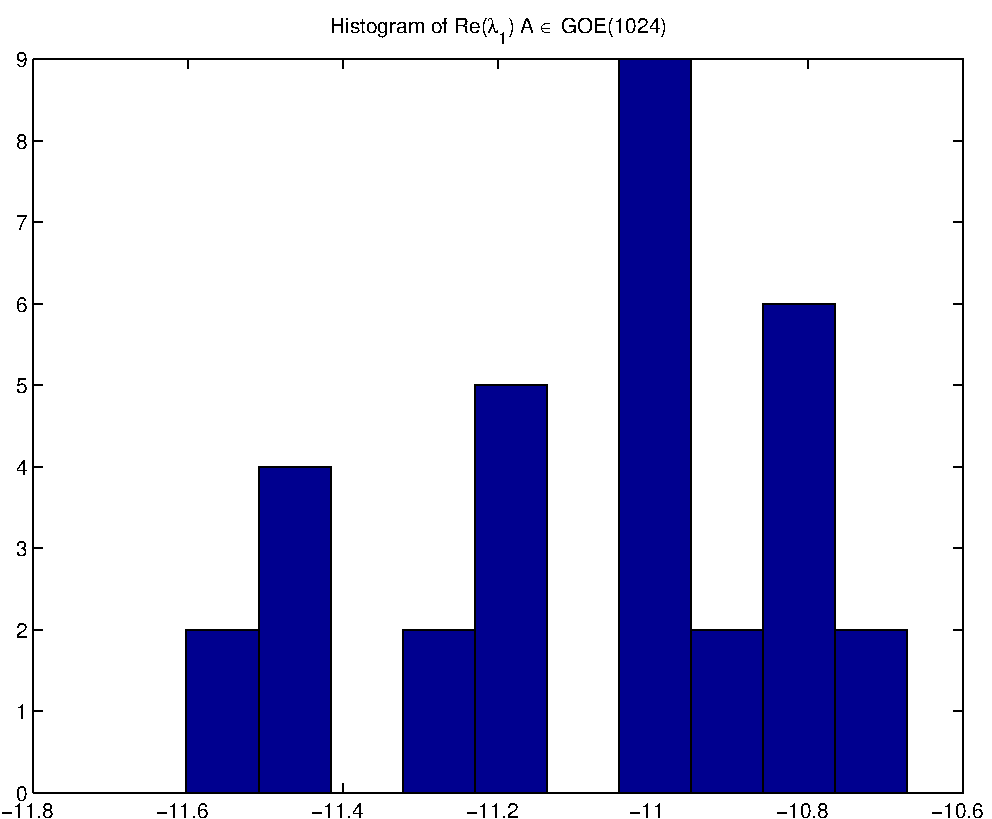
\includegraphics[width=10.0cm,height=10.0cm]{Re_Winger.pdf}

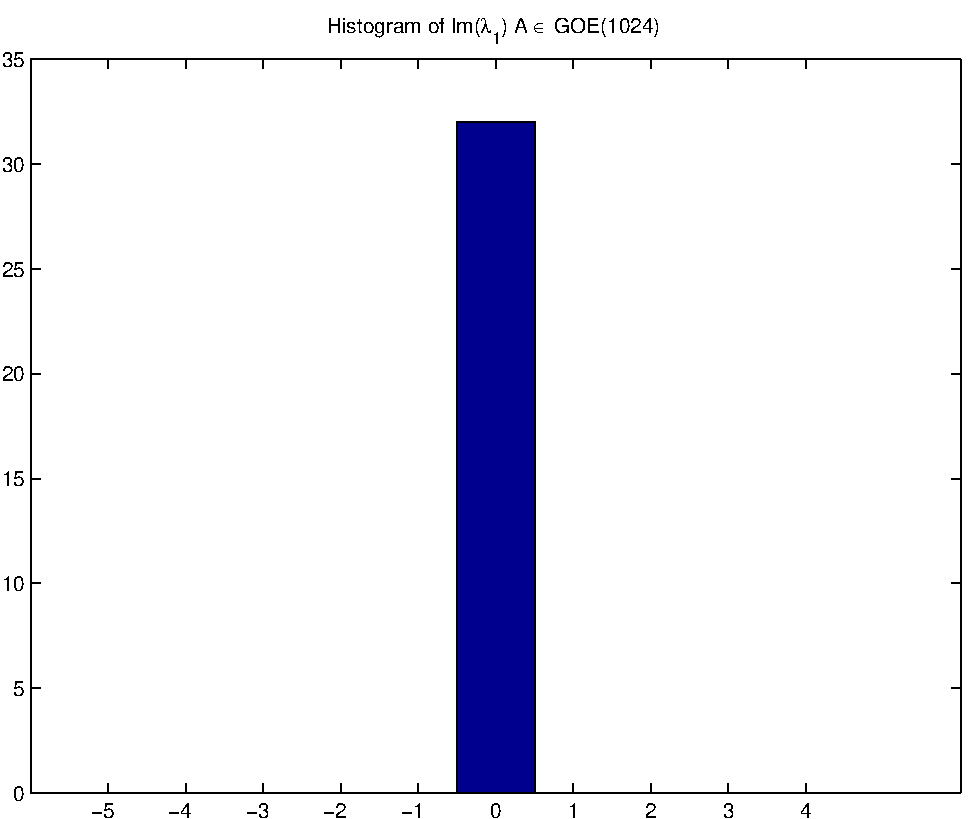
\includegraphics[width=10.0cm,height=10.0cm]{Im_Winger.pdf}

QueryPerformanceCounter  =  +7.926
\subsubsection{Approximate Winger Distribution}
\subsubsection{Verfy Winger Law.}
Let $M_n = [X_{ij} ]$ a symmetric n x n matrix with Random entries such that $X_{i,j} = X_{j,i}$, 		  and $X_{i,j}$ are iid $orall i < j,$ and $Xjj$ are iid $orall j  :  ; E[X^2_{ij} ] = 1, & E[X_{ij}] = 0$ 		  and that all moments exists for each of the entries.  		  The eigenvector of this random matrix; $ lambda_1 leq ... leq lambda_n$ depends continuously on $Mn$.
Dimension $n = +512$

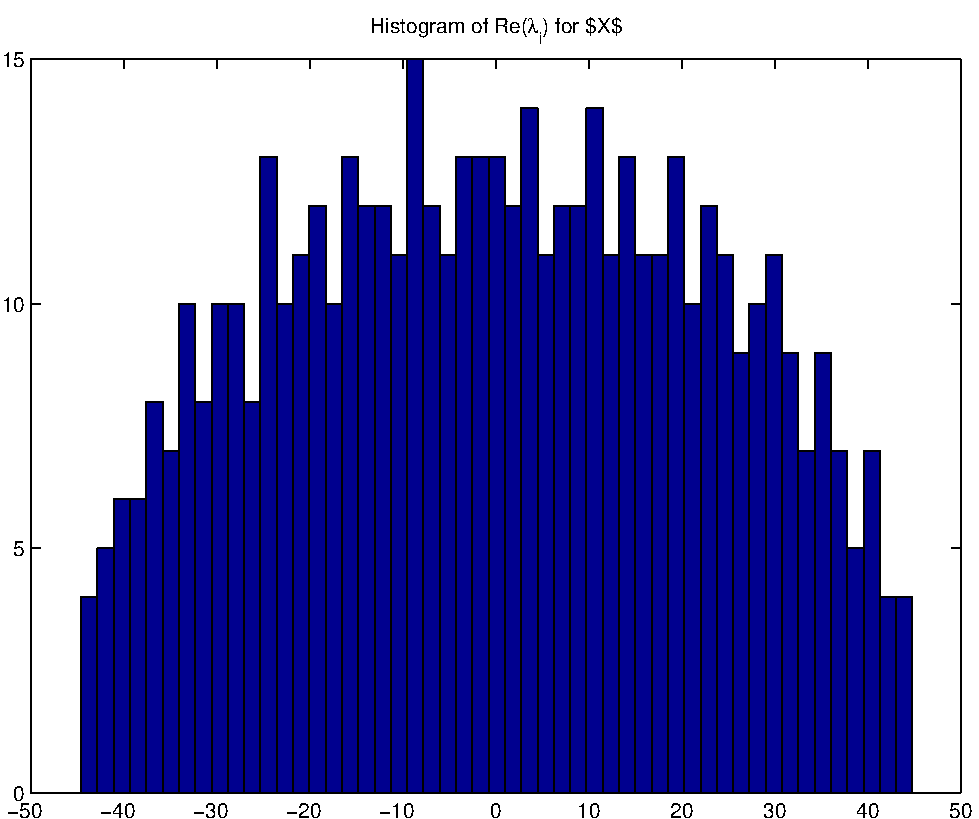
\includegraphics[width=10.0cm,height=10.0cm]{Re_lambda_n.pdf}

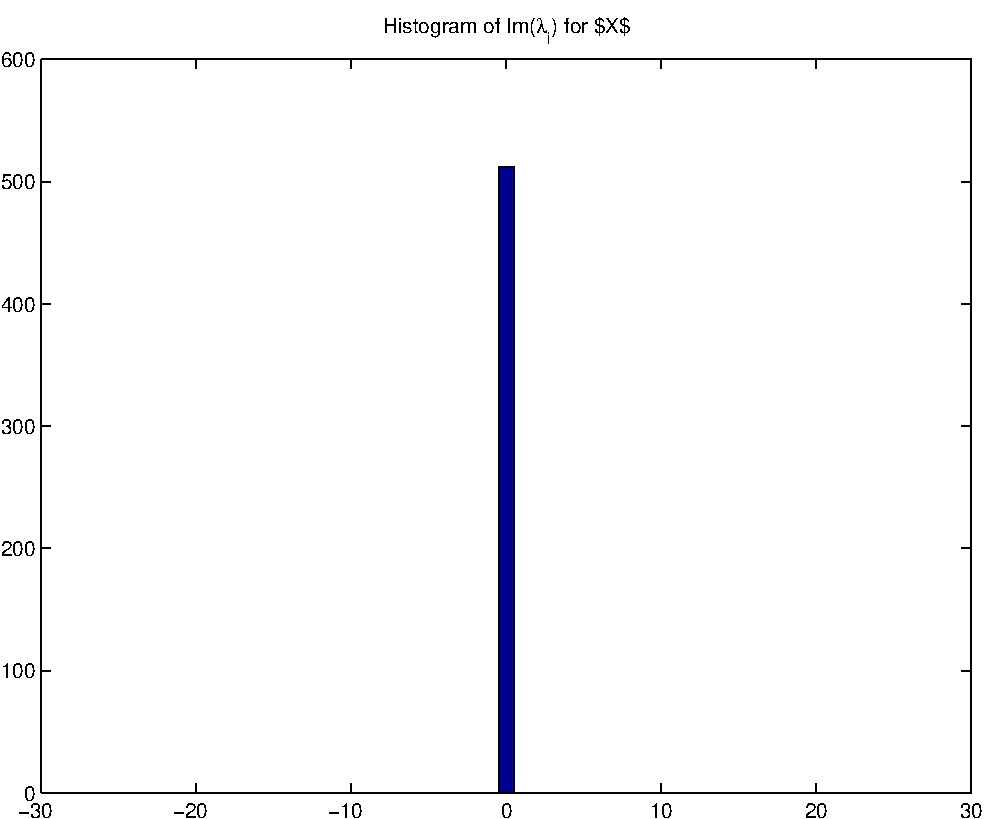
\includegraphics[width=10.0cm,height=10.0cm]{Im_lambda_n.pdf}

QueryPerformanceCounter  =  +2.673
\subsubsection{Matrix Exponential }
$SPD Matrix = \left(
\begin{array}{
cccccccc}
+10.539 & -0.499 & -0.010 & +0.368 & +0.465 & -0.492 & -0.126 & +0.437 \\
-0.499 & +7.286 & +0.365 & -0.481 & -0.337 & -0.466 & +0.279 & +0.056 \\
-0.010 & +0.365 & +6.705 & -0.205 & +0.467 & +0.131 & +0.077 & -0.089 \\
+0.368 & -0.481 & -0.205 & +6.496 & -0.402 & -0.209 & +0.043 & -0.041 \\
+0.465 & -0.337 & +0.467 & -0.402 & +4.578 & +0.272 & +0.289 & -0.285 \\
-0.492 & -0.466 & +0.131 & -0.209 & +0.272 & +8.181 & +0.343 & -0.244 \\
-0.126 & +0.279 & +0.077 & +0.043 & +0.289 & +0.343 & +5.938 & -0.212 \\
+0.437 & +0.056 & -0.089 & -0.041 & -0.285 & -0.244 & -0.212 & +9.691 \\
\end{array}
\right)$ \newline 

$SPD Eigs = \left(
\begin{array}{
cccccccc}
(+10.93611,+0.00000) & (+9.60778,+0.00000) & (+4.23666,+0.00000) & (+8.36911,+0.00000) & (+7.56229,+0.00000) & (+5.82791,+0.00000) & (+6.54198,+0.00000) & (+6.33139,+0.00000) \\
\end{array}
\right)$ \newline 

$exp(SPD) = \left(
\begin{array}{
cccccccc}
+47863.969 & -6460.093 & -1078.770 & +4706.958 & +2535.224 & -8475.398 & -2406.368 & +12977.552 \\
-6460.093 & +2780.574 & +516.920 & -1069.918 & -548.083 & -109.707 & +386.466 & -807.216 \\
-1078.770 & +516.920 & +1015.281 & -385.755 & +176.069 & +458.541 & +212.284 & -859.022 \\
+4706.958 & -1069.918 & -385.755 & +1267.210 & +111.181 & -1018.272 & -287.809 & +1036.628 \\
+2535.224 & -548.083 & +176.069 & +111.181 & +413.265 & +135.193 & +45.490 & -502.411 \\
-8475.398 & -109.707 & +458.541 & -1018.272 & +135.193 & +5613.026 & +968.003 & -4270.737 \\
-2406.368 & +386.466 & +212.284 & -287.809 & +45.490 & +968.003 & +632.432 & -1645.725 \\
+12977.552 & -807.216 & -859.022 & +1036.628 & -502.411 & -4270.737 & -1645.725 & +19362.944 \\
\end{array}
\right)$ \newline 

$exp(SPD) eigs = \left(
\begin{array}{
cccccccc}
(+56168.17045,+0.00000) & (+14880.07985,+0.00000) & (+4311.77579,+0.00000) & (+1924.25027,+0.00000) & (+69.17669,+0.00000) & (+339.64809,+0.00000) & (+693.66208,+0.00000) & (+561.93669,+0.00000) \\
\end{array}
\right)$ \newline 

$log(exp(SPD) eigs)  = \left(
\begin{array}{
cccccccc}
(+10.93611,+0.00000) & (+9.60778,+0.00000) & (+8.36911,+0.00000) & (+7.56229,+0.00000) & (+4.23666,+0.00000) & (+5.82791,+0.00000) & (+6.54198,+0.00000) & (+6.33139,+0.00000) \\
\end{array}
\right)$ \newline 

$exp(Id) = \left(
\begin{array}{
cccccccc}
+2.718 & +0.000 & +0.000 & +0.000 & +0.000 & +0.000 & +0.000 & +0.000 \\
+0.000 & +2.718 & +0.000 & +0.000 & +0.000 & +0.000 & +0.000 & +0.000 \\
+0.000 & +0.000 & +2.718 & +0.000 & +0.000 & +0.000 & +0.000 & +0.000 \\
+0.000 & +0.000 & +0.000 & +2.718 & +0.000 & +0.000 & +0.000 & +0.000 \\
+0.000 & +0.000 & +0.000 & +0.000 & +2.718 & +0.000 & +0.000 & +0.000 \\
+0.000 & +0.000 & +0.000 & +0.000 & +0.000 & +2.718 & +0.000 & +0.000 \\
+0.000 & +0.000 & +0.000 & +0.000 & +0.000 & +0.000 & +2.718 & +0.000 \\
+0.000 & +0.000 & +0.000 & +0.000 & +0.000 & +0.000 & +0.000 & +2.718 \\
\end{array}
\right)$ \newline 

$exp(Id) eigs = \left(
\begin{array}{
cccccccc}
(+2.71828,+0.00000) & (+2.71828,+0.00000) & (+2.71828,+0.00000) & (+2.71828,+0.00000) & (+2.71828,+0.00000) & (+2.71828,+0.00000) & (+2.71828,+0.00000) & (+2.71828,+0.00000) \\
\end{array}
\right)$ \newline 

$log(exp(Id) eigs)  = \left(
\begin{array}{
cccccccc}
(+1.00000,+0.00000) & (+1.00000,+0.00000) & (+1.00000,+0.00000) & (+1.00000,+0.00000) & (+1.00000,+0.00000) & (+1.00000,+0.00000) & (+1.00000,+0.00000) & (+1.00000,+0.00000) \\
\end{array}
\right)$ \newline 

For $n  \in  \dblz [16,128)$ we calculate  $|( SPD(n) Eigs - log(exp(SPD(n)) eigs)|_{l^2}$

$|( SPD(n) Eigs - log(exp(SPD(n)) eigs)|_{l^2} = \left(
\begin{array}{
cccccccccccccccccccccccccccccccccccccccccccccccccccccccccccccccccccccccccccccccccccccccccccccccccccccccccccccccc}
(+5.36543,+0.00000) & (+5.36543,+0.00000) & (+5.36543,+0.00000) & (+5.36543,+0.00000) & (+5.36543,+0.00000) & (+5.36543,+0.00000) & (+5.36543,+0.00000) & (+5.36543,+0.00000) & (+5.36543,+0.00000) & (+5.36543,+0.00000) & (+5.36543,+0.00000) & (+5.36543,+0.00000) & (+5.36543,+0.00000) & (+5.36543,+0.00000) & (+5.36543,+0.00000) & (+5.36543,+0.00000) & (+5.36543,+0.00000) & (+5.36543,+0.00000) & (+5.36543,+0.00000) & (+5.36543,+0.00000) & (+5.36543,+0.00000) & (+5.36543,+0.00000) & (+5.36543,+0.00000) & (+5.36543,+0.00000) & (+5.36543,+0.00000) & (+5.36543,+0.00000) & (+5.36543,+0.00000) & (+5.36543,+0.00000) & (+5.36543,+0.00000) & (+5.36543,+0.00000) & (+5.36543,+0.00000) & (+5.36543,+0.00000) & (+5.36543,+0.00000) & (+5.36543,+0.00000) & (+5.36543,+0.00000) & (+5.36543,+0.00000) & (+5.36543,+0.00000) & (+5.36543,+0.00000) & (+5.36543,+0.00000) & (+5.36543,+0.00000) & (+5.36543,+0.00000) & (+5.36543,+0.00000) & (+5.36543,+0.00000) & (+5.36543,+0.00000) & (+5.36543,+0.00000) & (+5.36543,+0.00000) & (+5.36543,+0.00000) & (+5.36543,+0.00000) & (-0.00000,-0.00000) & (-0.00000,-0.00000) & (-0.00000,-0.00000) & (-0.00000,-0.00000) & (-0.00000,-0.00000) & (-0.00000,-0.00000) & (-0.00000,-0.00000) & (-0.00000,-0.00000) & (-0.00000,-0.00000) & (-0.00000,-0.00000) & (-0.00000,-0.00000) & (-0.00000,-0.00000) & (-0.00000,-0.00000) & (-0.00000,-0.00000) & (-0.00000,-0.00000) & (-0.00000,-0.00000) & (-0.00000,-0.00000) & (-0.00000,-0.00000) & (-0.00000,-0.00000) & (-0.00000,-0.00000) & (-0.00000,-0.00000) & (-0.00000,-0.00000) & (-0.00000,-0.00000) & (-0.00000,-0.00000) & (-0.00000,-0.00000) & (-0.00000,-0.00000) & (-0.00000,-0.00000) & (-0.00000,-0.00000) & (-0.00000,-0.00000) & (-0.00000,-0.00000) & (-0.00000,-0.00000) & (-0.00000,-0.00000) & (-0.00000,-0.00000) & (-0.00000,-0.00000) & (-0.00000,-0.00000) & (-0.00000,-0.00000) & (-0.00000,-0.00000) & (-0.00000,-0.00000) & (-0.00000,-0.00000) & (-0.00000,-0.00000) & (-0.00000,-0.00000) & (-0.00000,-0.00000) & (-0.00000,-0.00000) & (-0.00000,-0.00000) & (-0.00000,-0.00000) & (-0.00000,-0.00000) & (-0.00000,-0.00000) & (-0.00000,-0.00000) & (-0.00000,-0.00000) & (-0.00000,-0.00000) & (-0.00000,-0.00000) & (-0.00000,-0.00000) & (-0.00000,-0.00000) & (-0.00000,-0.00000) & (-0.00000,-0.00000) & (-0.00000,-0.00000) & (-0.00000,-0.00000) & (-0.00000,-0.00000) & (-0.00000,-0.00000) & (-0.00000,-0.00000) & (-0.00000,-0.00000) & (-0.00000,-0.00000) & (-0.00000,-0.00000) & (-0.00000,-0.00000) \\
\end{array}
\right)$ \newline 

QueryPerformanceCounter  =  +0.04407
The sample size generated for this run is 100000.

\newpage
uniform \begin{tabular}{|c|c|c|c|}  mean & variance & skewness & kurtosis \\  \hline
$\mu_1 = +0.50030$ & $\mu_2 = +0.08353$ & $\mu_3 = +0.00339$ & $\mu_4 =+1.80113$ \\
\end{tabular}

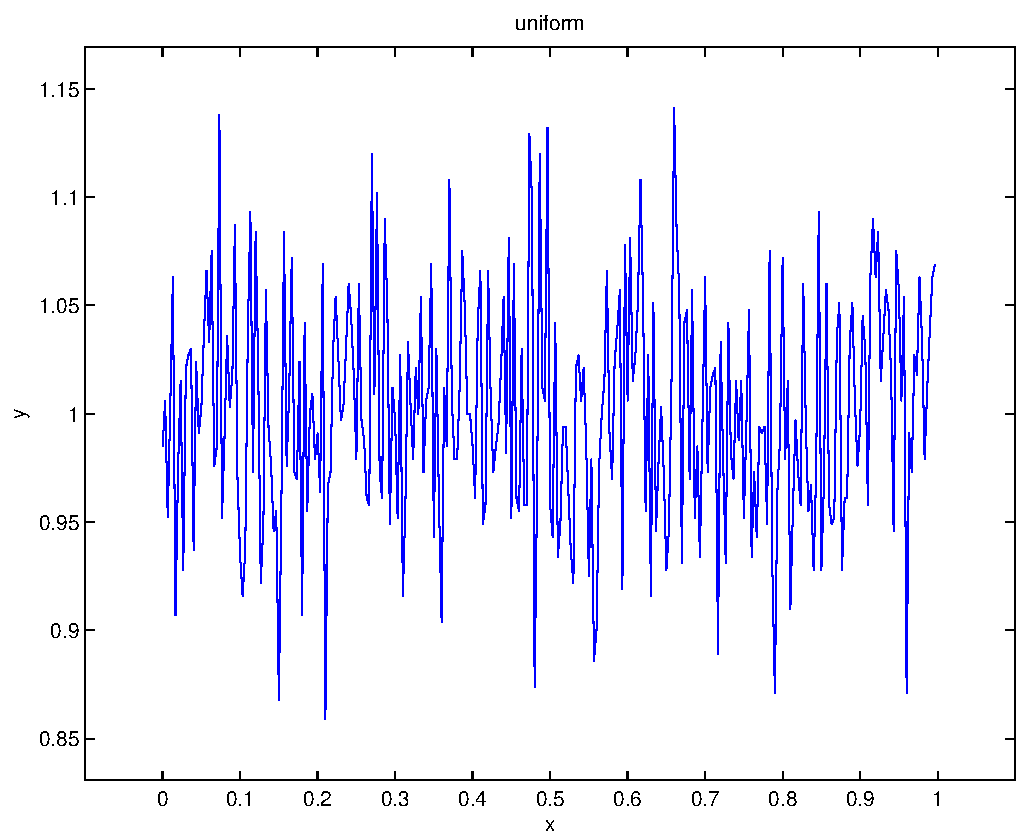
\includegraphics[width=5cm,height=5cm]{uniform.pdf}

cauchy \begin{tabular}{|c|c|c|c|}  mean & variance & skewness & kurtosis \\  \hline
$\mu_1 = +0.44288$ & $\mu_2 = +0.05341$ & $\mu_3 = +0.63935$ & $\mu_4 =+3.28094$ \\
\end{tabular}

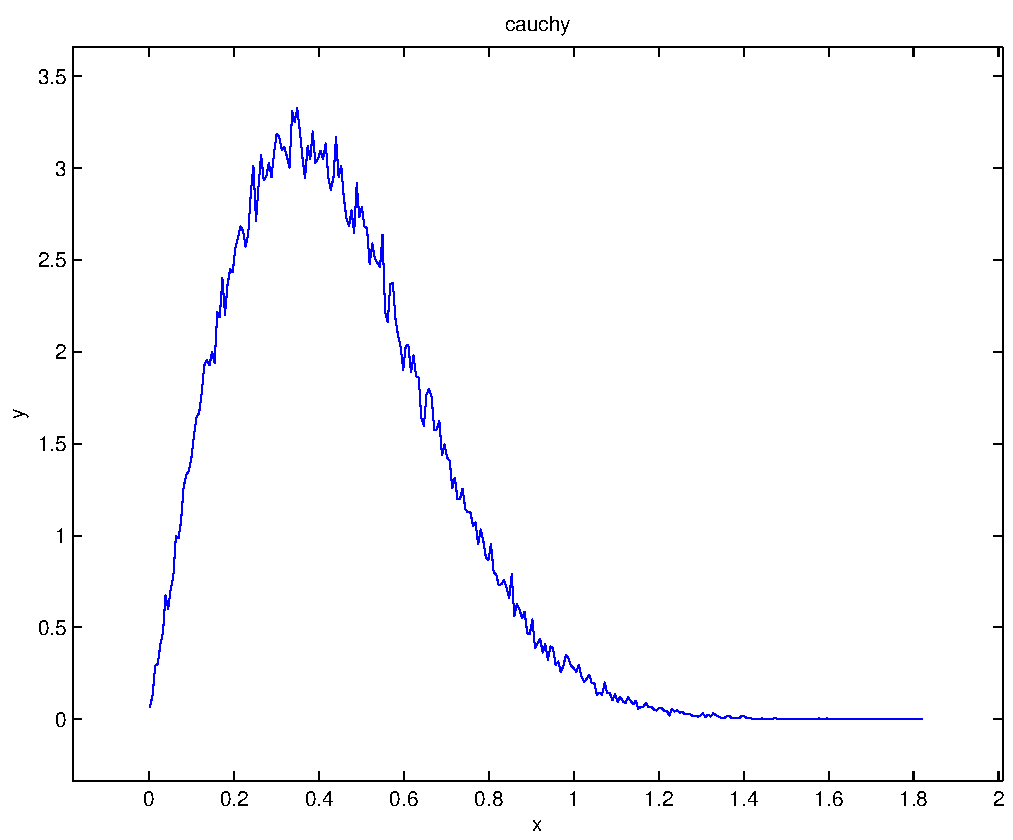
\includegraphics[width=5cm,height=5cm]{cauchy.pdf}

exponential \begin{tabular}{|c|c|c|c|}  mean & variance & skewness & kurtosis \\  \hline
$\mu_1 = +1.99647$ & $\mu_2 = +3.99339$ & $\mu_3 = +2.03097$ & $\mu_4 =+9.30842$ \\
\end{tabular}

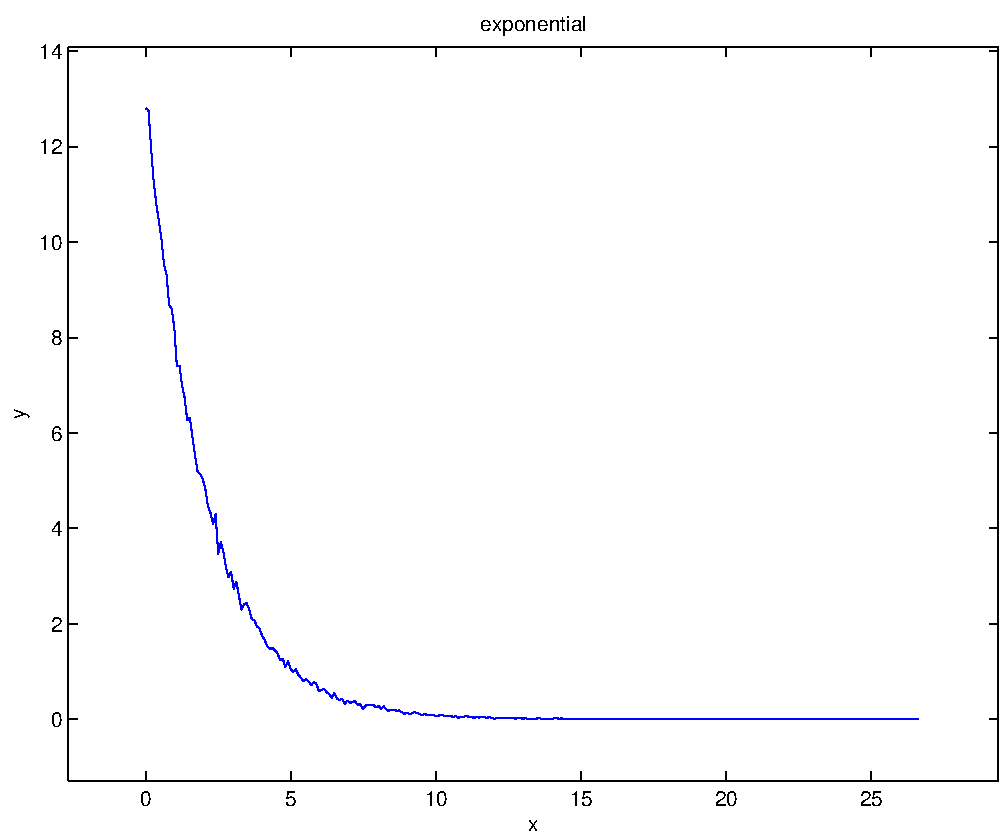
\includegraphics[width=5cm,height=5cm]{exponential.pdf}

\newpage
gamma \begin{tabular}{|c|c|c|c|}  mean & variance & skewness & kurtosis \\  \hline
$\mu_1 = +1.89991$ & $\mu_2 = +1.89577$ & $\mu_3 = +1.45616$ & $\mu_4 =+6.28140$ \\
\end{tabular}

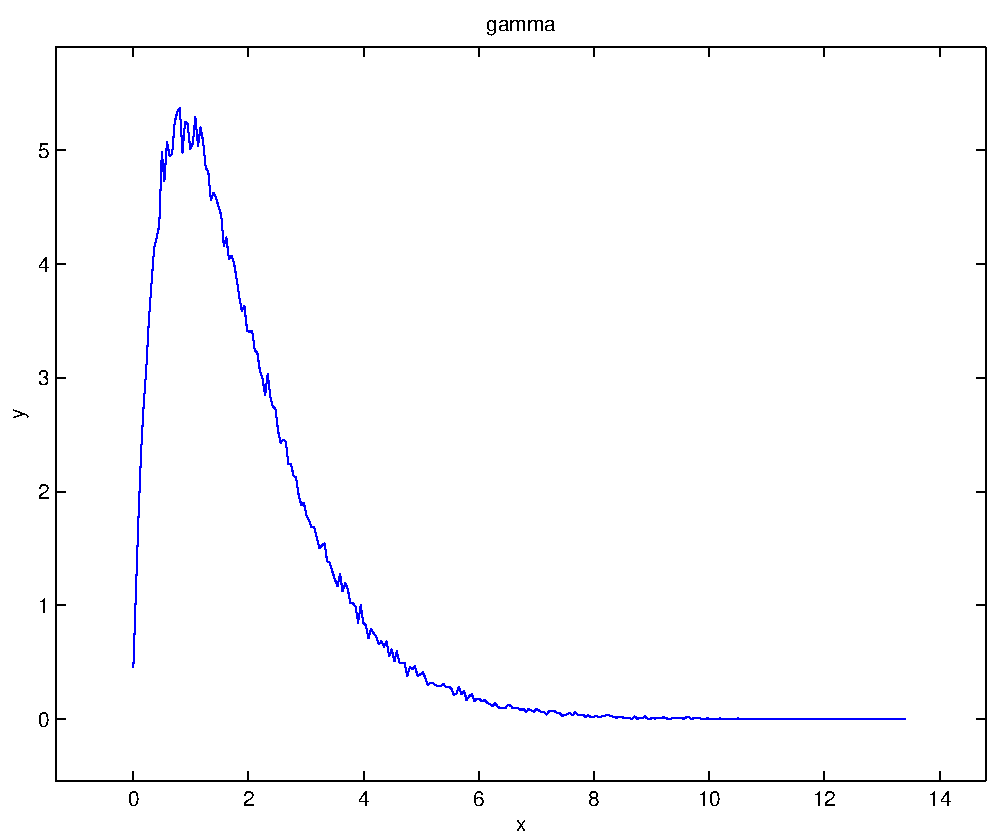
\includegraphics[width=5cm,height=5cm]{gamma.pdf}

GIG \begin{tabular}{|c|c|c|c|}  mean & variance & skewness & kurtosis \\  \hline
$\mu_1 = +0.82571$ & $\mu_2 = +12.30331$ & $\mu_3 = +14.83339$ & $\mu_4 =+291.47640$ \\
\end{tabular}

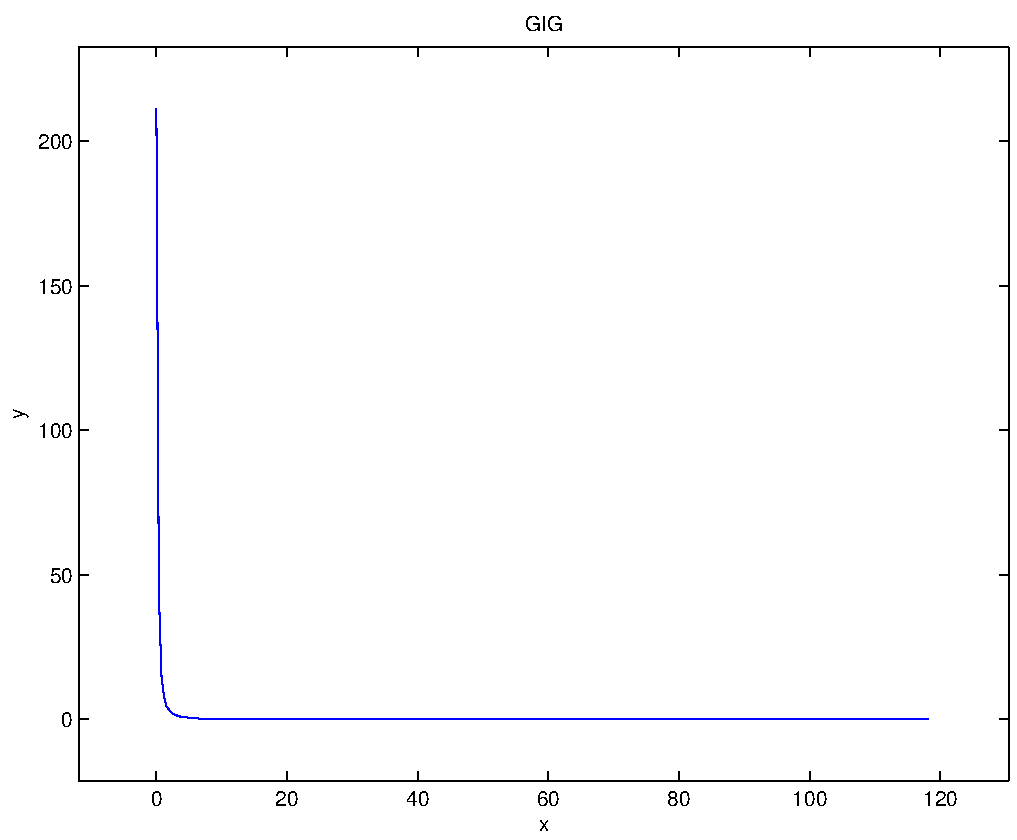
\includegraphics[width=5cm,height=5cm]{GIG.pdf}

normal-box-muller \begin{tabular}{|c|c|c|c|}  mean & variance & skewness & kurtosis \\  \hline
$\mu_1 = +0.00262$ & $\mu_2 = +0.99471$ & $\mu_3 = -0.00751$ & $\mu_4 =+2.97905$ \\
\end{tabular}

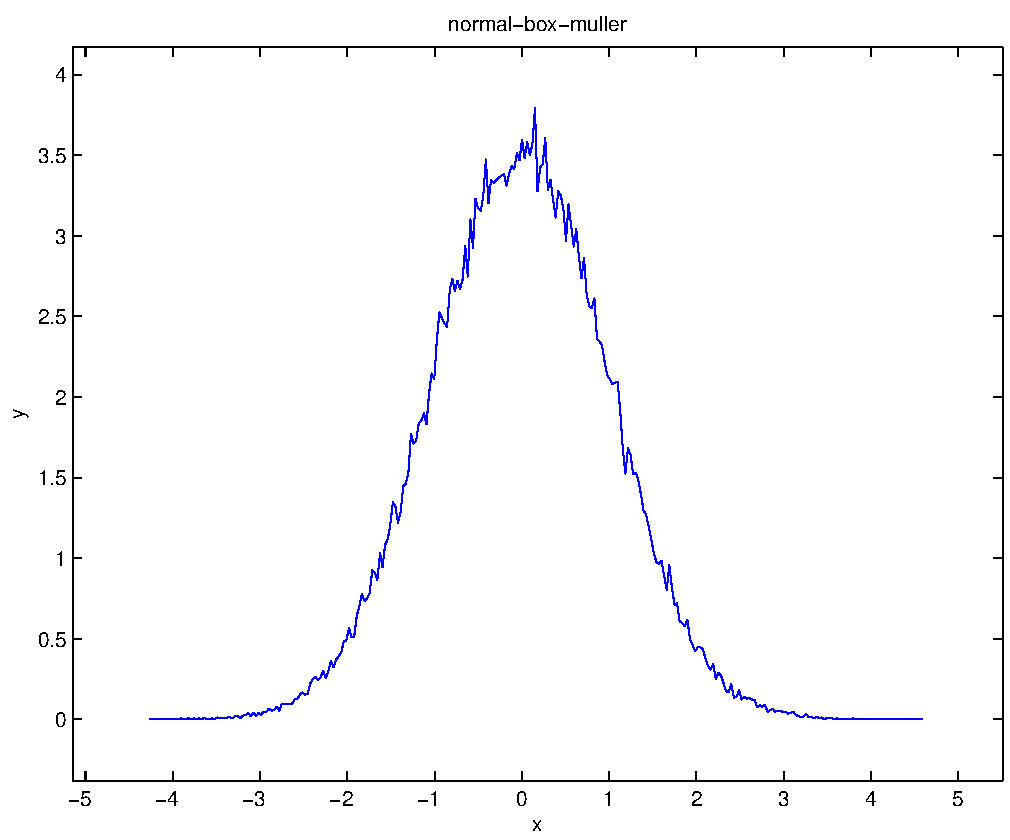
\includegraphics[width=5cm,height=5cm]{normal-box-muller.pdf}

\newpage
normal-inverse-approximation \begin{tabular}{|c|c|c|c|}  mean & variance & skewness & kurtosis \\  \hline
$\mu_1 = +0.00230$ & $\mu_2 = +1.00486$ & $\mu_3 = +0.01163$ & $\mu_4 =+2.99254$ \\
\end{tabular}

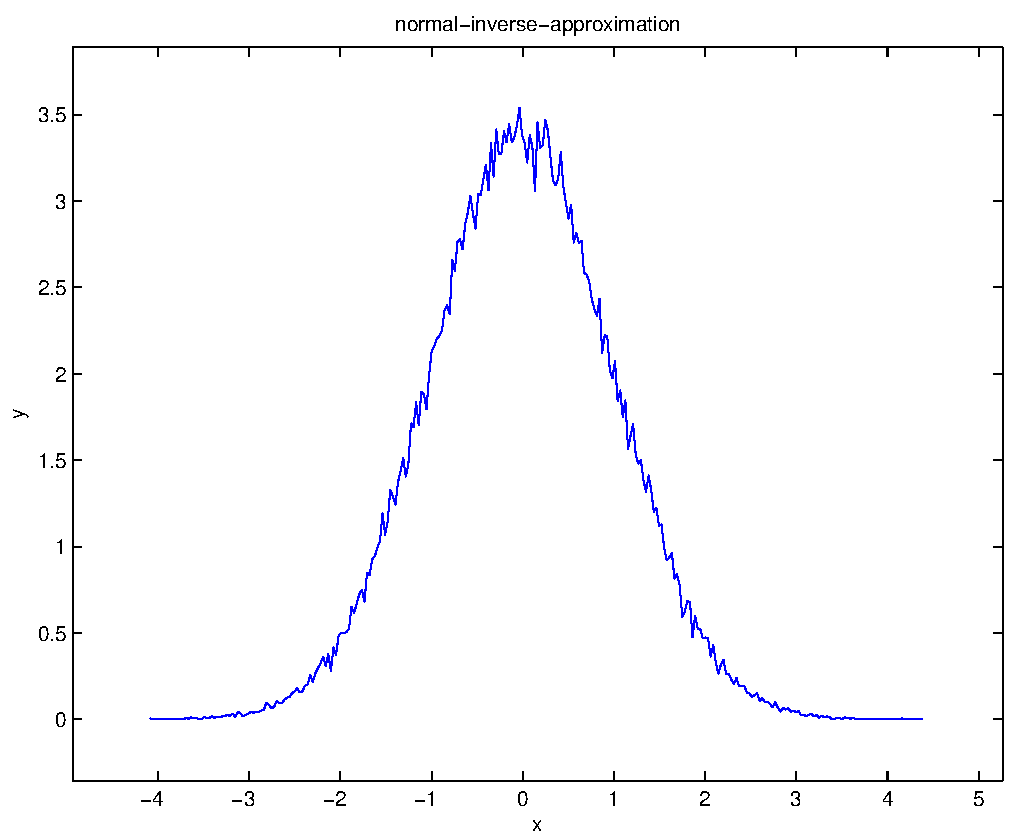
\includegraphics[width=5cm,height=5cm]{normal-inverse-approximation.pdf}

pareto \begin{tabular}{|c|c|c|c|}  mean & variance & skewness & kurtosis \\  \hline
$\mu_1 = +3184578.26493$ & $\mu_2 = +888468246174112900.00000$ & $\mu_3 = +315.36997$ & $\mu_4 =+99629.09819$ \\
\end{tabular}

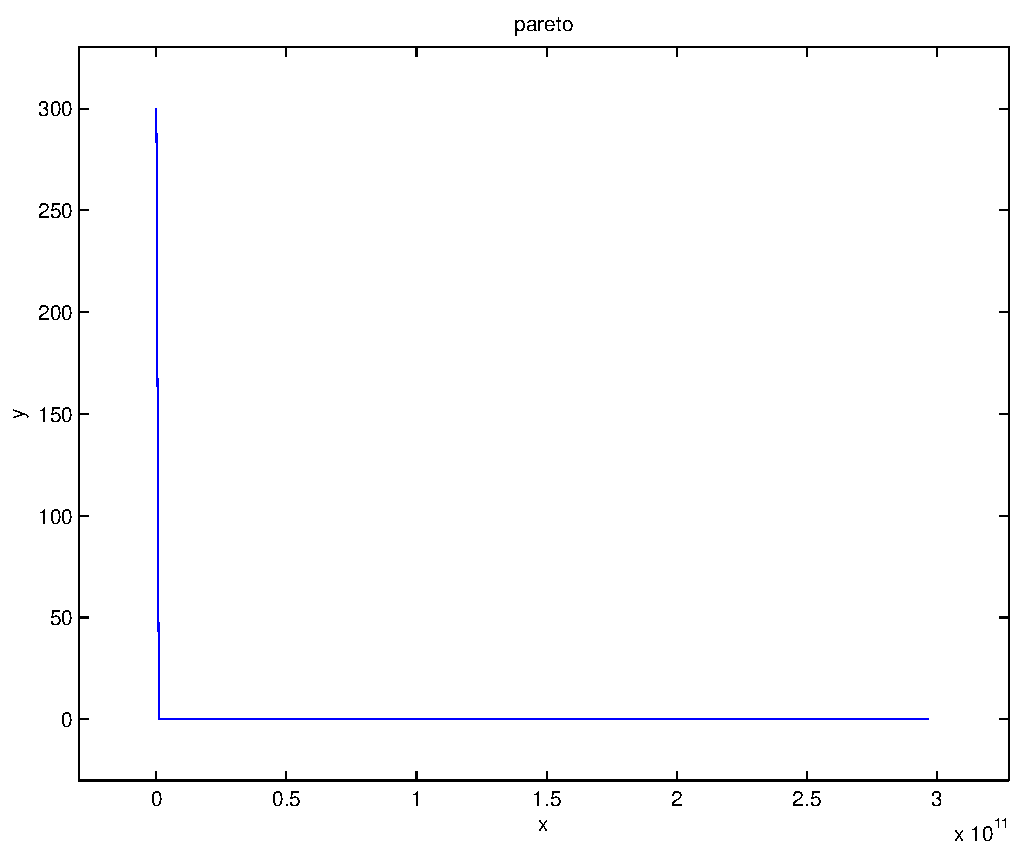
\includegraphics[width=5cm,height=5cm]{pareto.pdf}

poisson \begin{tabular}{|c|c|c|c|}  mean & variance & skewness & kurtosis \\  \hline
$\mu_1 = +1.10472$ & $\mu_2 = +0.12949$ & $\mu_3 = +3.95698$ & $\mu_4 =+21.59641$ \\
\end{tabular}

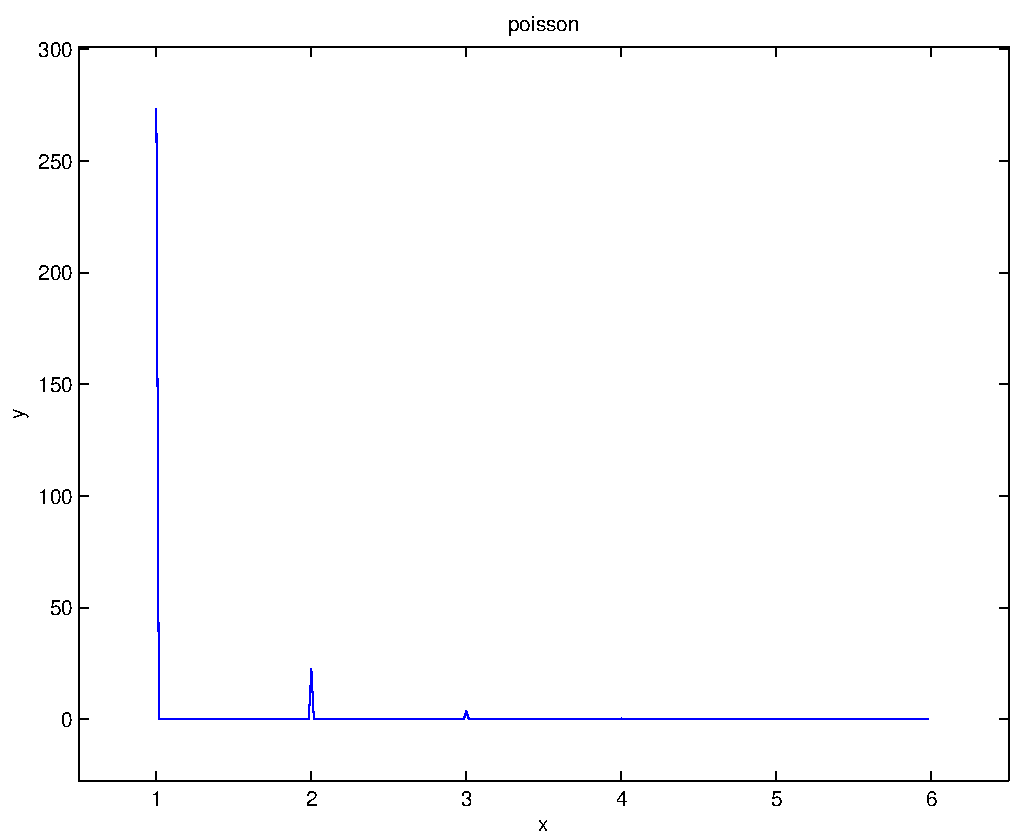
\includegraphics[width=5cm,height=5cm]{poisson.pdf}

\newpage
beta \begin{tabular}{|c|c|c|c|}  mean & variance & skewness & kurtosis \\  \hline
$\mu_1 = +0.33160$ & $\mu_2 = +0.12686$ & $\mu_3 = +0.68923$ & $\mu_4 =+1.91928$ \\
\end{tabular}

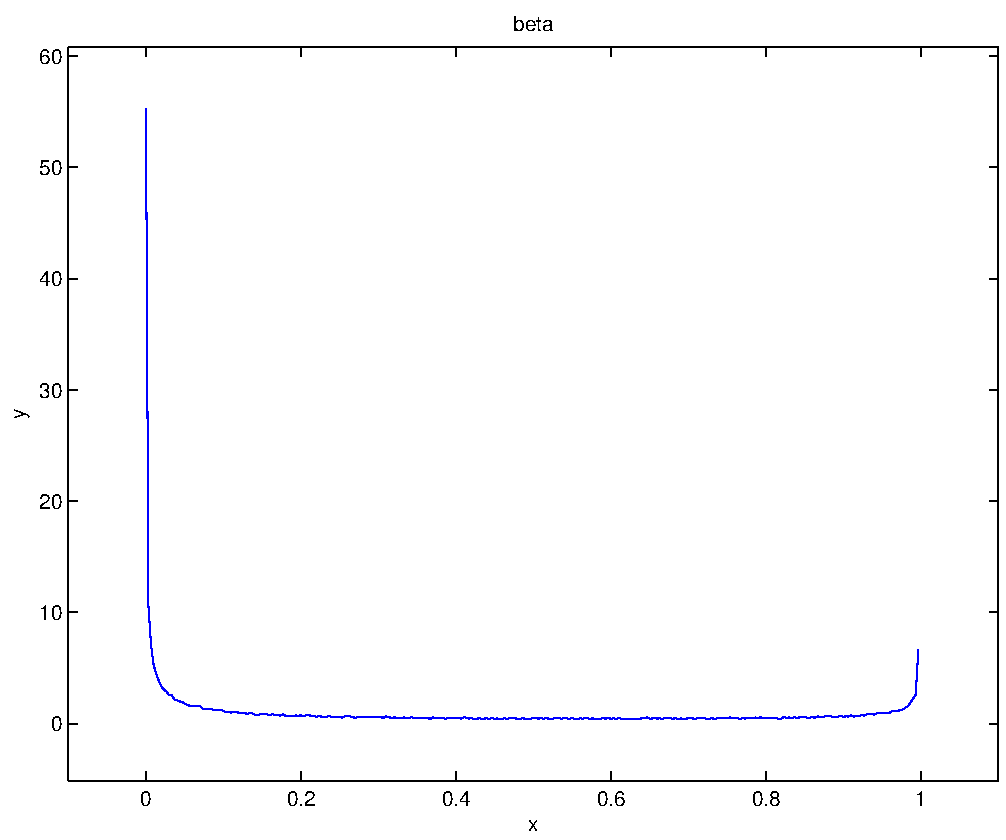
\includegraphics[width=5cm,height=5cm]{beta.pdf}

QueryPerformanceCounter  =  +21.38910
\subsubsection{Multiclass Support Vector Machine }
\begin{itemize}
\item Number or training points = 1024
\item Feature dimension = 3
\item Number or classes = 3
\end{itemize}
{The mean vectors of the 3 classes}

$\mu_1 = \left(
\begin{array}{
ccc}
+1.90000 & +0.10000 & +0.10000 \\
\end{array}
\right)$ \newline 

$\mu_2 = \left(
\begin{array}{
ccc}
+0.10000 & +1.90000 & +0.10000 \\
\end{array}
\right)$ \newline 

$\mu_3 = \left(
\begin{array}{
ccc}
+0.00000 & +0.00000 & +1.90000 \\
\end{array}
\right)$ \newline 

A random SPD covairance matrix is generated for each of the classes.\newline

$\rho_1 = \left(
\begin{array}{
ccc}
+1.767 & -0.184 & -0.435 \\
-0.184 & +3.573 & +0.289 \\
-0.435 & +0.289 & +2.231 \\
\end{array}
\right)$ \newline 

$\rho_2 = \left(
\begin{array}{
ccc}
+3.230 & +0.087 & -0.015 \\
+0.087 & +2.316 & -0.377 \\
-0.015 & -0.377 & +2.230 \\
\end{array}
\right)$ \newline 

$\rho_3 = \left(
\begin{array}{
ccc}
+2.357 & +0.205 & -0.491 \\
+0.205 & +1.804 & -0.395 \\
-0.491 & -0.395 & +1.764 \\
\end{array}
\right)$ \newline 

Verify $L_1$ condition number of covariance. The diagonal entries of the matrix have the form $(0.5 + U(0,1) )*dim(Dom(Cov))$
The lower-diagonal entries take the form $U(0,1) - 0.5$. 
The $L_1$ condition numbers are :
\begin{itemize}
\item +2.958
\item +1.786
\item +2.663
\end{itemize}
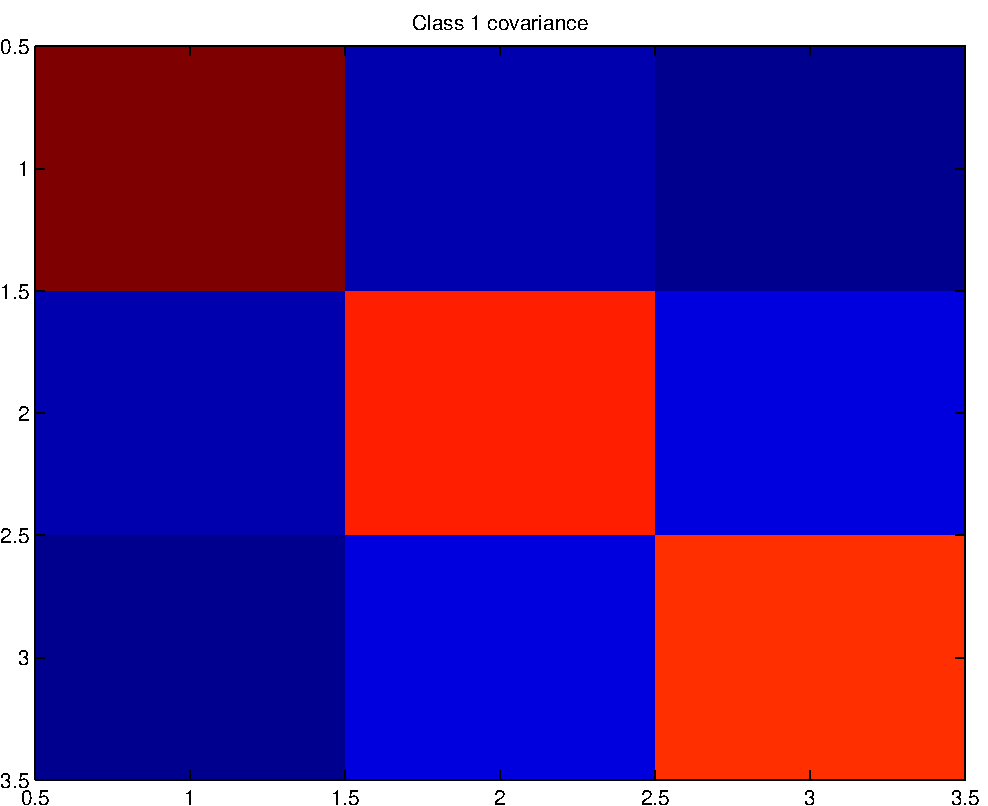
\includegraphics[width=10.0cm,height=10.0cm]{rv1_corr.pdf}

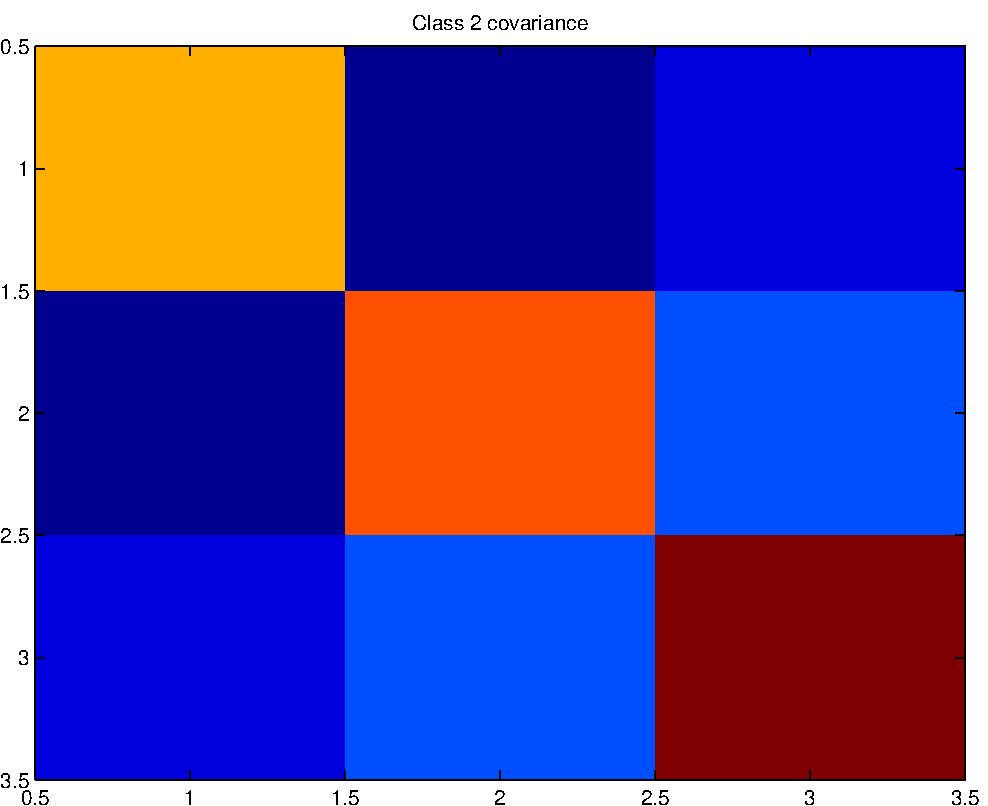
\includegraphics[width=10.0cm,height=10.0cm]{rv2_corr.pdf}

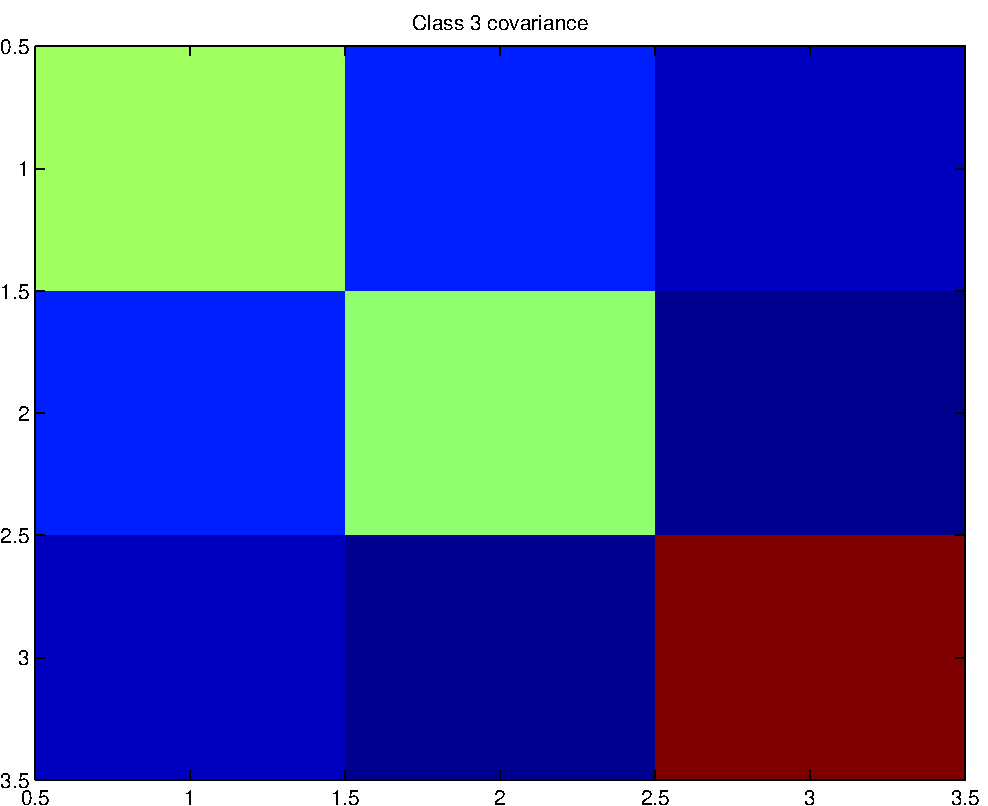
\includegraphics[width=10.0cm,height=10.0cm]{rv3_corr.pdf}

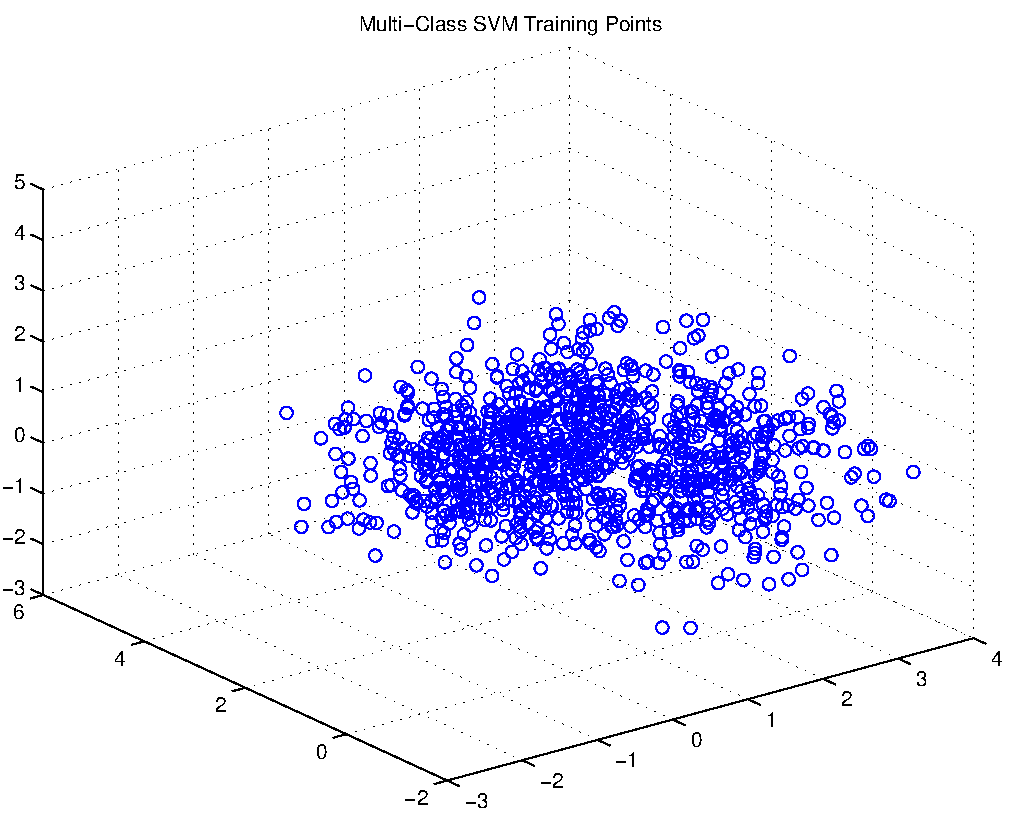
\includegraphics[width=10.0cm,height=10.0cm]{trainingPoints.pdf}

These are the SVM parameters - the RBF kernel is used\begin{itemize}
\item allOutlierFraction=0.05
\item mixingCoeff=0.3
\item smoThresh=1.0/10000.0
\item sigma=1
\end{itemize}
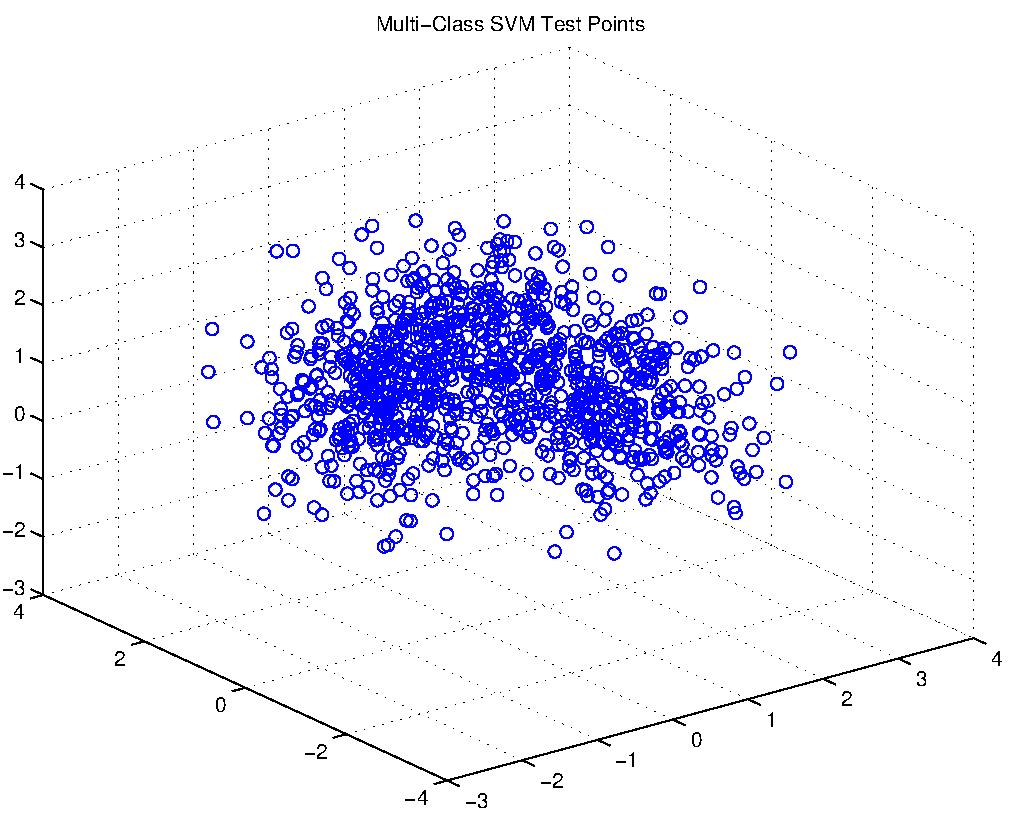
\includegraphics[width=10.0cm,height=10.0cm]{testPoints.pdf}

The marginal sample moments (mean var skew kurtosis) for training points.\newline
\begin{tabular}{ c |  c  c  c  c}
Feature & $\mu_1$ & $\mu_2$ & $\mu_3$ & $\mu_4$ \\
0 & +0.668 & +1.259 & +0.115& +2.162 \\
\hline
1 & +0.699 & +1.208 & +0.309& +2.265 \\
\hline
2 & +0.695 & +1.124 & +0.327& +2.256 \\
\hline
\end{tabular}
\newline
The marginal sample moments (mean var skew kurtosis) for test points.\newline
\begin{tabular}{ c | c  c  c  c}
Feature & $\mu_1$ & $\mu_2$ & $\mu_3$ & $\mu_4$ \\
0 & +0.676 & +1.165 & +0.258& +2.165\\
\hline
1 & +0.665 & +1.209 & +0.345& +2.269\\
\hline
2 & +0.714 & +1.084 & +0.313& +2.185\\
\hline
\end{tabular}\newline
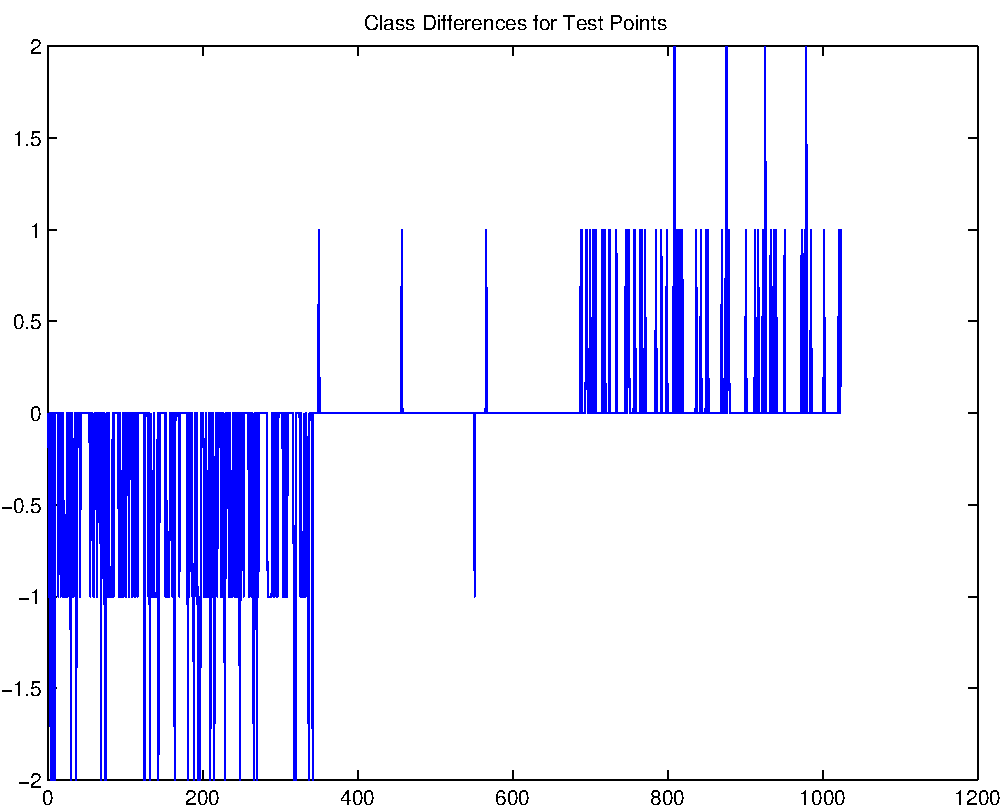
\includegraphics[width=10.0cm,height=10.0cm]{classDiffs.pdf}

The error rate for this run is +0.085\newline
QueryPerformanceCounter  =  +6.495
\subsubsection{Semidefinite Programming SDPA}
QueryPerformanceCounter  =  +0.038
\subsubsection{Linear Regression 3x1}
\subsubsection{3 x 1 Linear Regression}
Sample size = 64

Number of features = 3

$\sigma = \left(
\begin{array}{
ccc}
+3.952 & -0.499 & -0.010 \\
-0.499 & +1.895 & +0.465 \\
-0.010 & +0.465 & +4.477 \\
\end{array}
\right)$ \newline 

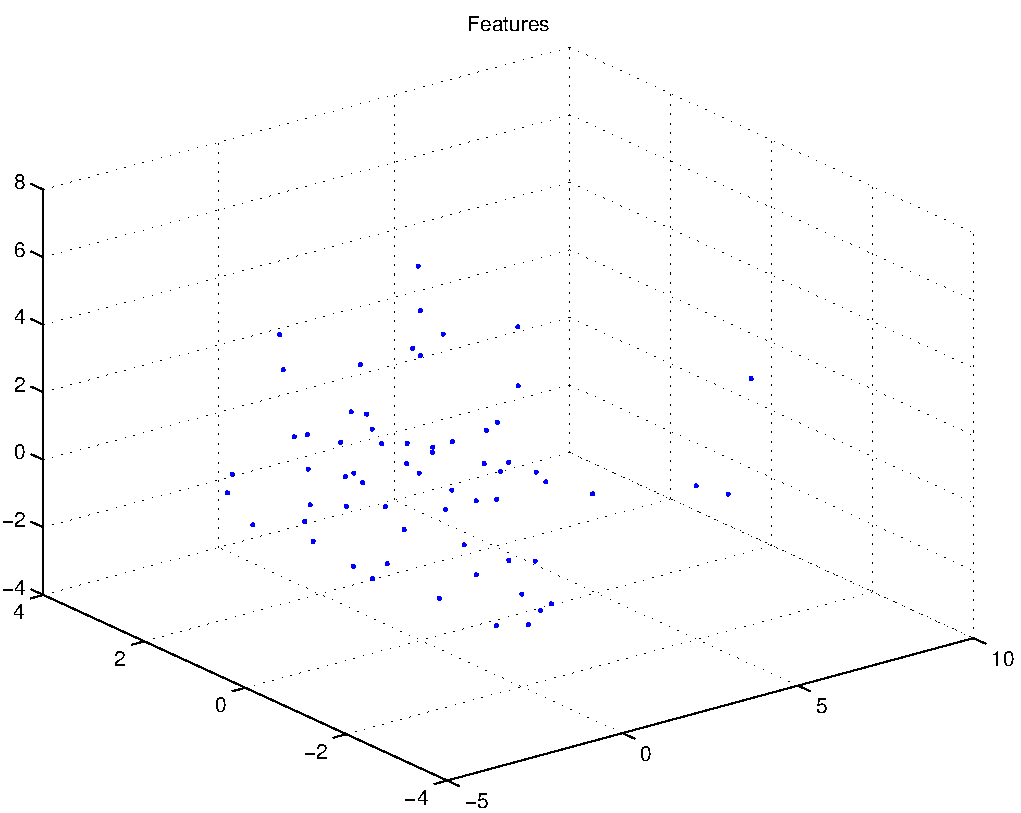
\includegraphics[width=10.0cm,height=10.0cm]{regression_features.pdf}

Beta
+0.817, +0.999, +0.510

Response
+2.055
+2.409
+2.279
+4.677
-0.124
+6.800
+0.758
+2.409
+3.712
+0.491
-1.916
+1.016
+0.259
+3.514
+1.649
+2.369
+1.563
+2.251
+2.336
+2.078
+0.286
+4.669
-0.056
+0.352
+1.067
+2.313
-1.281
-3.493
-3.672
+1.303
+0.836
+0.167
-2.268
+1.992
+2.259
+3.923
+1.769
+5.004
+1.434
-1.199
+6.134
+1.790
-2.201
+2.774
+2.724
-1.899
+1.982
-3.000
-2.350
-0.437
-0.375
-0.669
-2.274
+0.692
-0.883
-1.489
+0.164
+2.959
-2.551
-1.133
-3.392
+1.514
-2.036
+0.904
Estimate for Beta
-6277438562204192200000000000000000000000000000000000000000000000000.000
-6277438562204192200000000000000000000000000000000000000000000000000.000
-6277438562204192200000000000000000000000000000000000000000000000000.000
Error:
-0.000, -0.000, -0.000


QueryPerformanceCounter  =  +1.063
\subsubsection{Matrix Norms}
\subsubsection{Haar Distributed Random Orthogonal Matrix $A \in O(n)$}
 Testing Operator Norm
Number of Dimensions: +12

$A = \left(
\begin{array}{
cccccccccccc}
+0.007 & -0.301 & -0.301 & +0.094 & -0.058 & +0.403 & -0.158 & -0.082 & +0.416 & +0.279 & +0.491 & +0.346 \\
+0.782 & +0.199 & -0.018 & -0.272 & +0.155 & -0.224 & +0.060 & -0.178 & +0.030 & -0.098 & +0.392 & -0.026 \\
-0.304 & -0.029 & -0.036 & -0.144 & +0.833 & -0.017 & +0.165 & -0.328 & -0.132 & +0.078 & +0.047 & +0.172 \\
-0.038 & +0.100 & -0.176 & +0.132 & -0.222 & -0.570 & -0.280 & -0.262 & -0.274 & +0.379 & -0.060 & +0.444 \\
+0.141 & +0.308 & +0.272 & +0.602 & +0.236 & +0.248 & -0.198 & +0.276 & -0.369 & +0.111 & +0.255 & +0.058 \\
-0.052 & +0.357 & +0.012 & -0.561 & +0.109 & +0.076 & -0.218 & +0.579 & +0.090 & +0.235 & -0.099 & +0.285 \\
-0.179 & +0.059 & +0.073 & -0.121 & -0.225 & +0.089 & +0.162 & -0.005 & -0.266 & -0.643 & +0.258 & +0.556 \\
+0.258 & +0.381 & -0.397 & +0.267 & +0.068 & +0.263 & +0.195 & -0.132 & +0.212 & -0.128 & -0.537 & +0.283 \\
+0.340 & -0.516 & +0.547 & +0.025 & +0.112 & +0.006 & -0.055 & +0.038 & +0.094 & +0.022 & -0.366 & +0.397 \\
+0.155 & -0.362 & -0.400 & +0.069 & +0.039 & -0.125 & +0.536 & +0.484 & -0.333 & +0.164 & +0.026 & +0.057 \\
-0.119 & +0.299 & +0.424 & +0.040 & -0.207 & -0.034 & +0.652 & -0.101 & +0.231 & +0.390 & +0.137 & +0.112 \\
+0.137 & -0.033 & +0.012 & -0.332 & -0.222 & +0.549 & +0.017 & -0.331 & -0.548 & +0.294 & -0.129 & -0.074 \\
\end{array}
\right)$ \newline 

$Det(A) :   A \in O(n)$ = (+1.000,+0.000)

$L = \left(
\begin{array}{
cccccccccccc}
+1.000 & +0.000 & +0.000 & +0.000 & +0.000 & +0.000 & +0.000 & +0.000 & +0.000 & +0.000 & +0.000 & +0.000 \\
+0.435 & +1.000 & +0.000 & +0.000 & +0.000 & +0.000 & +0.000 & +0.000 & +0.000 & +0.000 & +0.000 & +0.000 \\
+0.198 & +0.667 & +1.000 & +0.000 & +0.000 & +0.000 & +0.000 & +0.000 & +0.000 & +0.000 & +0.000 & +0.000 \\
+0.181 & -0.452 & -0.685 & +1.000 & +0.000 & +0.000 & +0.000 & +0.000 & +0.000 & +0.000 & +0.000 & +0.000 \\
-0.389 & -0.080 & -0.001 & -0.324 & +1.000 & +0.000 & +0.000 & +0.000 & +0.000 & +0.000 & +0.000 & +0.000 \\
+0.176 & +0.113 & +0.062 & -0.411 & -0.171 & +1.000 & +0.000 & +0.000 & +0.000 & +0.000 & +0.000 & +0.000 \\
-0.152 & -0.546 & -0.944 & +0.140 & -0.217 & -0.280 & +1.000 & +0.000 & +0.000 & +0.000 & +0.000 & +0.000 \\
-0.066 & -0.615 & -0.459 & -0.652 & +0.285 & +0.315 & +0.007 & +1.000 & +0.000 & +0.000 & +0.000 & +0.000 \\
+0.009 & +0.503 & +0.756 & +0.005 & -0.068 & +0.683 & -0.490 & -0.241 & +1.000 & +0.000 & +0.000 & +0.000 \\
-0.049 & -0.183 & +0.099 & +0.194 & -0.254 & -0.880 & -0.204 & -0.378 & -0.957 & +1.000 & +0.000 & +0.000 \\
+0.330 & -0.524 & +0.131 & +0.583 & -0.084 & +0.403 & -0.036 & -0.315 & +0.876 & -0.398 & +1.000 & +0.000 \\
-0.229 & -0.173 & -0.215 & -0.208 & -0.147 & +0.100 & +0.283 & +0.101 & -0.304 & -0.596 & -0.509 & +1.000 \\
\end{array}
\right)$ \newline 

$U = \left(
\begin{array}{
cccccccccccc}
+0.782 & +0.199 & -0.018 & -0.272 & +0.155 & -0.224 & +0.060 & -0.178 & +0.030 & -0.098 & +0.392 & -0.026 \\
+0.000 & -0.602 & +0.555 & +0.143 & +0.044 & +0.104 & -0.081 & +0.116 & +0.081 & +0.064 & -0.536 & +0.409 \\
+0.000 & +0.000 & -0.767 & +0.027 & -0.022 & -0.150 & +0.578 & +0.442 & -0.393 & +0.140 & +0.306 & -0.210 \\
+0.000 & +0.000 & +0.000 & +0.734 & +0.213 & +0.232 & +0.151 & +0.664 & -0.607 & +0.254 & +0.152 & +0.103 \\
+0.000 & +0.000 & +0.000 & +0.000 & +0.966 & -0.021 & +0.231 & -0.172 & -0.311 & +0.127 & +0.206 & +0.228 \\
+0.000 & +0.000 & +0.000 & +0.000 & +0.000 & +0.678 & +0.082 & -0.097 & -0.841 & +0.421 & -0.058 & -0.021 \\
+0.000 & +0.000 & +0.000 & +0.000 & +0.000 & +0.000 & +1.214 & +0.195 & -0.310 & +0.653 & +0.200 & +0.161 \\
+0.000 & +0.000 & +0.000 & +0.000 & +0.000 & +0.000 & +0.000 & +1.353 & -0.078 & +0.324 & -0.206 & +0.446 \\
+0.000 & +0.000 & +0.000 & +0.000 & +0.000 & +0.000 & +0.000 & +0.000 & +1.058 & +0.260 & +0.627 & +0.516 \\
+0.000 & +0.000 & +0.000 & +0.000 & +0.000 & +0.000 & +0.000 & +0.000 & +0.000 & +1.230 & +0.366 & +1.253 \\
+0.000 & +0.000 & +0.000 & +0.000 & +0.000 & +0.000 & +0.000 & +0.000 & +0.000 & +0.000 & -1.496 & +0.694 \\
+0.000 & +0.000 & +0.000 & +0.000 & +0.000 & +0.000 & +0.000 & +0.000 & +0.000 & +0.000 & +0.000 & +1.799 \\
\end{array}
\right)$ \newline 

$L * U  = \left(
\begin{array}{
cccccccccccc}
+0.782 & +0.199 & -0.018 & -0.272 & +0.155 & -0.224 & +0.060 & -0.178 & +0.030 & -0.098 & +0.392 & -0.026 \\
+0.340 & -0.516 & +0.547 & +0.025 & +0.112 & +0.006 & -0.055 & +0.038 & +0.094 & +0.022 & -0.366 & +0.397 \\
+0.155 & -0.362 & -0.400 & +0.069 & +0.039 & -0.125 & +0.536 & +0.484 & -0.333 & +0.164 & +0.026 & +0.057 \\
+0.141 & +0.308 & +0.272 & +0.602 & +0.236 & +0.248 & -0.198 & +0.276 & -0.369 & +0.111 & +0.255 & +0.058 \\
-0.304 & -0.029 & -0.036 & -0.144 & +0.833 & -0.017 & +0.165 & -0.328 & -0.132 & +0.078 & +0.047 & +0.172 \\
+0.137 & -0.033 & +0.012 & -0.332 & -0.222 & +0.549 & +0.017 & -0.331 & -0.548 & +0.294 & -0.129 & -0.074 \\
-0.119 & +0.299 & +0.424 & +0.040 & -0.207 & -0.034 & +0.652 & -0.101 & +0.231 & +0.390 & +0.137 & +0.112 \\
-0.052 & +0.357 & +0.012 & -0.561 & +0.109 & +0.076 & -0.218 & +0.579 & +0.090 & +0.235 & -0.099 & +0.285 \\
+0.007 & -0.301 & -0.301 & +0.094 & -0.058 & +0.403 & -0.158 & -0.082 & +0.416 & +0.279 & +0.491 & +0.346 \\
-0.038 & +0.100 & -0.176 & +0.132 & -0.222 & -0.570 & -0.280 & -0.262 & -0.274 & +0.379 & -0.060 & +0.444 \\
+0.258 & +0.381 & -0.397 & +0.267 & +0.068 & +0.263 & +0.195 & -0.132 & +0.212 & -0.128 & -0.537 & +0.283 \\
-0.179 & +0.059 & +0.073 & -0.121 & -0.225 & +0.089 & +0.162 & -0.005 & -0.266 & -0.643 & +0.258 & +0.556 \\
\end{array}
\right)$ \newline 

$Det(L) :    = (+1.000,+0.000)     Det(U) :    = (-1.000,+0.000)     Det(LU) :    = (-1.000,-0.000)$

$||A||_{L_1}$  = +2.995

$||A||_{L_{\infty}}$ = +3.122

$||A^{-1}||_{L_1}$  = +3.122

$||A^{-1}||_{L_{\infty}}$ = +2.995

$||A||_{L_{\infty}} * ||A^{-1}||_{L_{\infty}} = +9.350$

$||A||_{L_1} * ||A^{-1}||_{L_1} = +9.350$

Frobenious Norm  $||A||_{\textit{F}}$ via $\sum\limits_{i,j =0}^{n} \|A_{i,j}|$   of  $A \in O(n)$  +3.464

$L_1$ condition number of Haar Distributed Random Orthogonal Matrix $A \in O(n)$ +8.023

$A = \left(
\begin{array}{
cccccccccccc}
+0.007 & -0.301 & -0.301 & +0.094 & -0.058 & +0.403 & -0.158 & -0.082 & +0.416 & +0.279 & +0.491 & +0.346 \\
+0.782 & +0.199 & -0.018 & -0.272 & +0.155 & -0.224 & +0.060 & -0.178 & +0.030 & -0.098 & +0.392 & -0.026 \\
-0.304 & -0.029 & -0.036 & -0.144 & +0.833 & -0.017 & +0.165 & -0.328 & -0.132 & +0.078 & +0.047 & +0.172 \\
-0.038 & +0.100 & -0.176 & +0.132 & -0.222 & -0.570 & -0.280 & -0.262 & -0.274 & +0.379 & -0.060 & +0.444 \\
+0.141 & +0.308 & +0.272 & +0.602 & +0.236 & +0.248 & -0.198 & +0.276 & -0.369 & +0.111 & +0.255 & +0.058 \\
-0.052 & +0.357 & +0.012 & -0.561 & +0.109 & +0.076 & -0.218 & +0.579 & +0.090 & +0.235 & -0.099 & +0.285 \\
-0.179 & +0.059 & +0.073 & -0.121 & -0.225 & +0.089 & +0.162 & -0.005 & -0.266 & -0.643 & +0.258 & +0.556 \\
+0.258 & +0.381 & -0.397 & +0.267 & +0.068 & +0.263 & +0.195 & -0.132 & +0.212 & -0.128 & -0.537 & +0.283 \\
+0.340 & -0.516 & +0.547 & +0.025 & +0.112 & +0.006 & -0.055 & +0.038 & +0.094 & +0.022 & -0.366 & +0.397 \\
+0.155 & -0.362 & -0.400 & +0.069 & +0.039 & -0.125 & +0.536 & +0.484 & -0.333 & +0.164 & +0.026 & +0.057 \\
-0.119 & +0.299 & +0.424 & +0.040 & -0.207 & -0.034 & +0.652 & -0.101 & +0.231 & +0.390 & +0.137 & +0.112 \\
+0.137 & -0.033 & +0.012 & -0.332 & -0.222 & +0.549 & +0.017 & -0.331 & -0.548 & +0.294 & -0.129 & -0.074 \\
\end{array}
\right)$ \newline 

$L_{\infty}$ condition number of Haar Distributed Random Orthogonal Matrix $A \in O(n)$ +7.760

Eigenvalues of $A \in O(n)$

(-1.000,+0.029), (-1.000,-0.029), (-0.602,+0.799), (-0.602,-0.799), (-0.072,+0.997), (-0.072,-0.997), (+0.415,+0.910), (+0.415,-0.910), (+0.743,+0.670), (+0.743,-0.670), (+0.998,+0.068), (+0.998,-0.068)

 $|\lambda | : \lambda \in \sigma(A) , A \in O(n)$

+1.000, +1.000, +1.000, +1.000, +1.000, +1.000, +1.000, +1.000, +1.000, +1.000, +1.000, +1.000


Calculating $A^{\dag} A,$  we expect $A^{\dag} A \approx I$

$A^{\dag} A = \left(
\begin{array}{
cccccccccccc}
+1.000 & -0.000 & -0.000 & +0.000 & -0.000 & +0.000 & -0.000 & +0.000 & +0.000 & +0.000 & +0.000 & -0.000 \\
-0.000 & +1.000 & +0.000 & -0.000 & +0.000 & -0.000 & -0.000 & +0.000 & -0.000 & +0.000 & +0.000 & +0.000 \\
-0.000 & +0.000 & +1.000 & +0.000 & -0.000 & -0.000 & +0.000 & +0.000 & +0.000 & -0.000 & -0.000 & +0.000 \\
+0.000 & -0.000 & +0.000 & +1.000 & +0.000 & +0.000 & +0.000 & +0.000 & -0.000 & -0.000 & +0.000 & -0.000 \\
-0.000 & +0.000 & -0.000 & +0.000 & +1.000 & +0.000 & -0.000 & +0.000 & +0.000 & -0.000 & -0.000 & -0.000 \\
+0.000 & -0.000 & -0.000 & +0.000 & +0.000 & +1.000 & -0.000 & +0.000 & +0.000 & +0.000 & +0.000 & -0.000 \\
-0.000 & -0.000 & +0.000 & +0.000 & -0.000 & -0.000 & +1.000 & -0.000 & -0.000 & +0.000 & +0.000 & +0.000 \\
+0.000 & +0.000 & +0.000 & +0.000 & +0.000 & +0.000 & -0.000 & +1.000 & +0.000 & +0.000 & -0.000 & +0.000 \\
+0.000 & -0.000 & +0.000 & -0.000 & +0.000 & +0.000 & -0.000 & +0.000 & +1.000 & -0.000 & -0.000 & +0.000 \\
+0.000 & +0.000 & -0.000 & -0.000 & -0.000 & +0.000 & +0.000 & +0.000 & -0.000 & +1.000 & +0.000 & -0.000 \\
+0.000 & +0.000 & -0.000 & +0.000 & -0.000 & +0.000 & +0.000 & -0.000 & -0.000 & +0.000 & +1.000 & +0.000 \\
-0.000 & +0.000 & +0.000 & -0.000 & -0.000 & -0.000 & +0.000 & +0.000 & +0.000 & -0.000 & +0.000 & +1.000 \\
\end{array}
\right)$ \newline 

Calculating $A^{-1} ,  A \in O(n)$.

$A^{-1} = \left(
\begin{array}{
cccccccccccc}
+0.007 & +0.782 & -0.304 & -0.038 & +0.141 & -0.052 & -0.179 & +0.258 & +0.340 & +0.155 & -0.119 & +0.137 \\
-0.301 & +0.199 & -0.029 & +0.100 & +0.308 & +0.357 & +0.059 & +0.381 & -0.516 & -0.362 & +0.299 & -0.033 \\
-0.301 & -0.018 & -0.036 & -0.176 & +0.272 & +0.012 & +0.073 & -0.397 & +0.547 & -0.400 & +0.424 & +0.012 \\
+0.094 & -0.272 & -0.144 & +0.132 & +0.602 & -0.561 & -0.121 & +0.267 & +0.025 & +0.069 & +0.040 & -0.332 \\
-0.058 & +0.155 & +0.833 & -0.222 & +0.236 & +0.109 & -0.225 & +0.068 & +0.112 & +0.039 & -0.207 & -0.222 \\
+0.403 & -0.224 & -0.017 & -0.570 & +0.248 & +0.076 & +0.089 & +0.263 & +0.006 & -0.125 & -0.034 & +0.549 \\
-0.158 & +0.060 & +0.165 & -0.280 & -0.198 & -0.218 & +0.162 & +0.195 & -0.055 & +0.536 & +0.652 & +0.017 \\
-0.082 & -0.178 & -0.328 & -0.262 & +0.276 & +0.579 & -0.005 & -0.132 & +0.038 & +0.484 & -0.101 & -0.331 \\
+0.416 & +0.030 & -0.132 & -0.274 & -0.369 & +0.090 & -0.266 & +0.212 & +0.094 & -0.333 & +0.231 & -0.548 \\
+0.279 & -0.098 & +0.078 & +0.379 & +0.111 & +0.235 & -0.643 & -0.128 & +0.022 & +0.164 & +0.390 & +0.294 \\
+0.491 & +0.392 & +0.047 & -0.060 & +0.255 & -0.099 & +0.258 & -0.537 & -0.366 & +0.026 & +0.137 & -0.129 \\
+0.346 & -0.026 & +0.172 & +0.444 & +0.058 & +0.285 & +0.556 & +0.283 & +0.397 & +0.057 & +0.112 & -0.074 \\
\end{array}
\right)$ \newline 

Calculating $A^{-1} *A  ,  A \in O(n)$.   We expect $A^{-1} *A  \approx I$. 

$A^{-1} *A = \left(
\begin{array}{
cccccccccccc}
+1.000 & +0.000 & -0.000 & -0.000 & -0.000 & +0.000 & +0.000 & +0.000 & -0.000 & +0.000 & +0.000 & +0.000 \\
-0.000 & +1.000 & -0.000 & -0.000 & -0.000 & +0.000 & -0.000 & +0.000 & +0.000 & -0.000 & +0.000 & +0.000 \\
+0.000 & -0.000 & +1.000 & -0.000 & -0.000 & +0.000 & -0.000 & -0.000 & +0.000 & -0.000 & -0.000 & -0.000 \\
+0.000 & +0.000 & +0.000 & +1.000 & -0.000 & +0.000 & +0.000 & +0.000 & -0.000 & +0.000 & -0.000 & +0.000 \\
-0.000 & -0.000 & +0.000 & -0.000 & +1.000 & +0.000 & +0.000 & -0.000 & -0.000 & -0.000 & +0.000 & +0.000 \\
-0.000 & +0.000 & +0.000 & +0.000 & -0.000 & +1.000 & +0.000 & +0.000 & -0.000 & -0.000 & -0.000 & -0.000 \\
+0.000 & -0.000 & +0.000 & +0.000 & +0.000 & +0.000 & +1.000 & -0.000 & +0.000 & +0.000 & -0.000 & +0.000 \\
+0.000 & -0.000 & -0.000 & -0.000 & -0.000 & +0.000 & +0.000 & +1.000 & -0.000 & -0.000 & +0.000 & -0.000 \\
+0.000 & +0.000 & +0.000 & +0.000 & -0.000 & +0.000 & +0.000 & -0.000 & +1.000 & -0.000 & +0.000 & +0.000 \\
+0.000 & +0.000 & -0.000 & -0.000 & -0.000 & -0.000 & +0.000 & -0.000 & -0.000 & +1.000 & +0.000 & -0.000 \\
+0.000 & +0.000 & +0.000 & -0.000 & +0.000 & -0.000 & +0.000 & -0.000 & -0.000 & +0.000 & +1.000 & -0.000 \\
+0.000 & -0.000 & +0.000 & -0.000 & +0.000 & -0.000 & +0.000 & +0.000 & +0.000 & -0.000 & -0.000 & +1.000 \\
\end{array}
\right)$ \newline 

Calculating SVD of  $A \in O(n)$

$U = \left(
\begin{array}{
cccccccccccc}
+0.049 & +0.445 & -0.337 & -0.171 & +0.043 & -0.375 & +0.179 & +0.053 & +0.189 & -0.104 & -0.084 & +0.653 \\
-0.007 & +0.301 & +0.301 & -0.094 & +0.058 & -0.403 & +0.158 & +0.082 & -0.416 & -0.279 & -0.491 & -0.346 \\
+0.252 & +0.333 & +0.609 & -0.015 & -0.065 & +0.150 & -0.484 & +0.327 & +0.093 & -0.052 & +0.126 & +0.241 \\
+0.131 & +0.024 & +0.372 & -0.253 & -0.548 & -0.121 & +0.290 & -0.576 & +0.062 & +0.058 & +0.199 & +0.050 \\
+0.192 & -0.176 & -0.383 & -0.357 & -0.479 & -0.152 & -0.399 & +0.188 & +0.063 & -0.394 & +0.024 & -0.225 \\
+0.243 & -0.487 & +0.165 & -0.145 & +0.236 & +0.221 & +0.243 & +0.004 & -0.206 & -0.556 & -0.021 & +0.374 \\
+0.202 & -0.281 & +0.035 & +0.508 & +0.060 & -0.475 & -0.430 & -0.384 & +0.001 & -0.019 & -0.170 & +0.175 \\
+0.380 & -0.095 & +0.004 & -0.568 & +0.400 & +0.028 & -0.159 & -0.194 & +0.199 & +0.380 & -0.326 & -0.101 \\
-0.227 & -0.437 & +0.277 & -0.008 & -0.215 & -0.252 & +0.205 & +0.437 & +0.444 & +0.179 & -0.316 & +0.093 \\
-0.546 & +0.069 & +0.013 & -0.110 & -0.141 & +0.384 & -0.298 & -0.326 & +0.063 & -0.177 & -0.497 & +0.199 \\
+0.107 & +0.189 & +0.051 & +0.199 & +0.207 & +0.070 & +0.146 & -0.161 & +0.700 & -0.462 & -0.000 & -0.335 \\
-0.523 & -0.108 & +0.179 & -0.342 & +0.365 & -0.382 & -0.210 & -0.083 & +0.040 & -0.138 & +0.462 & -0.037 \\
\end{array}
\right)$ \newline 

$S = \left(
\begin{array}{
cccccccccccc}
+1.000 & +0.000 & +0.000 & +0.000 & +0.000 & +0.000 & +0.000 & +0.000 & +0.000 & +0.000 & +0.000 & +0.000 \\
+0.000 & +1.000 & +0.000 & +0.000 & +0.000 & +0.000 & +0.000 & +0.000 & +0.000 & +0.000 & +0.000 & +0.000 \\
+0.000 & +0.000 & +1.000 & +0.000 & +0.000 & +0.000 & +0.000 & +0.000 & +0.000 & +0.000 & +0.000 & +0.000 \\
+0.000 & +0.000 & +0.000 & +1.000 & +0.000 & +0.000 & +0.000 & +0.000 & +0.000 & +0.000 & +0.000 & +0.000 \\
+0.000 & +0.000 & +0.000 & +0.000 & +1.000 & +0.000 & +0.000 & +0.000 & +0.000 & +0.000 & +0.000 & +0.000 \\
+0.000 & +0.000 & +0.000 & +0.000 & +0.000 & +1.000 & +0.000 & +0.000 & +0.000 & +0.000 & +0.000 & +0.000 \\
+0.000 & +0.000 & +0.000 & +0.000 & +0.000 & +0.000 & +1.000 & +0.000 & +0.000 & +0.000 & +0.000 & +0.000 \\
+0.000 & +0.000 & +0.000 & +0.000 & +0.000 & +0.000 & +0.000 & +1.000 & +0.000 & +0.000 & +0.000 & +0.000 \\
+0.000 & +0.000 & +0.000 & +0.000 & +0.000 & +0.000 & +0.000 & +0.000 & +1.000 & +0.000 & +0.000 & +0.000 \\
+0.000 & +0.000 & +0.000 & +0.000 & +0.000 & +0.000 & +0.000 & +0.000 & +0.000 & +1.000 & +0.000 & +0.000 \\
+0.000 & +0.000 & +0.000 & +0.000 & +0.000 & +0.000 & +0.000 & +0.000 & +0.000 & +0.000 & +1.000 & +0.000 \\
+0.000 & +0.000 & +0.000 & +0.000 & +0.000 & +0.000 & +0.000 & +0.000 & +0.000 & +0.000 & +0.000 & +1.000 \\
\end{array}
\right)$ \newline 

$V = \left(
\begin{array}{
cccccccccccc}
-0.000 & -1.000 & -0.000 & -0.000 & -0.000 & -0.000 & -0.000 & -0.000 & -0.000 & -0.000 & +0.000 & -0.000 \\
+0.237 & -0.000 & +0.176 & +0.304 & +0.177 & +0.161 & +0.053 & +0.358 & -0.440 & -0.632 & +0.195 & +0.000 \\
+0.139 & -0.000 & -0.319 & -0.221 & -0.588 & +0.235 & +0.006 & +0.309 & -0.255 & +0.102 & -0.006 & +0.507 \\
+0.423 & -0.000 & -0.052 & +0.174 & -0.018 & -0.341 & +0.584 & -0.045 & -0.059 & +0.026 & -0.568 & +0.042 \\
-0.219 & +0.000 & +0.509 & -0.364 & -0.439 & -0.064 & +0.097 & -0.357 & -0.348 & -0.246 & -0.129 & -0.169 \\
+0.404 & +0.000 & +0.473 & -0.305 & +0.102 & -0.152 & -0.491 & +0.344 & +0.169 & +0.074 & -0.286 & +0.106 \\
+0.357 & +0.000 & +0.144 & +0.224 & +0.117 & +0.578 & -0.169 & -0.555 & -0.170 & +0.215 & -0.120 & +0.169 \\
+0.486 & +0.000 & -0.129 & -0.196 & -0.149 & +0.039 & +0.056 & +0.078 & -0.168 & +0.287 & +0.328 & -0.677 \\
-0.101 & +0.000 & +0.337 & +0.084 & -0.189 & +0.560 & +0.389 & +0.318 & +0.477 & +0.036 & -0.097 & -0.169 \\
+0.094 & +0.000 & -0.471 & -0.287 & +0.002 & +0.250 & -0.199 & -0.133 & +0.235 & -0.545 & -0.387 & -0.254 \\
+0.157 & +0.000 & +0.032 & +0.573 & -0.588 & -0.234 & -0.321 & -0.125 & +0.296 & -0.158 & +0.083 & -0.085 \\
-0.357 & +0.000 & -0.084 & +0.310 & -0.037 & +0.096 & -0.282 & +0.284 & -0.400 & +0.267 & -0.504 & -0.338 \\
\end{array}
\right)$ \newline 

$U S V = \left(
\begin{array}{
cccccccccccc}
-0.360 & -0.049 & +0.114 & +0.508 & +0.225 & +0.373 & +0.020 & +0.094 & -0.438 & -0.054 & -0.030 & -0.450 \\
+0.057 & +0.007 & -0.183 & -0.214 & +0.197 & +0.082 & +0.293 & -0.167 & -0.604 & -0.026 & +0.508 & +0.367 \\
+0.138 & -0.252 & -0.169 & -0.060 & -0.461 & -0.052 & -0.029 & +0.767 & -0.253 & -0.056 & +0.100 & -0.063 \\
-0.143 & -0.131 & -0.325 & +0.413 & +0.008 & +0.383 & -0.284 & +0.085 & +0.210 & -0.008 & -0.010 & +0.638 \\
-0.213 & -0.192 & -0.060 & +0.126 & +0.302 & -0.257 & +0.044 & +0.195 & +0.408 & +0.291 & +0.648 & -0.176 \\
-0.196 & -0.243 & +0.289 & -0.063 & -0.198 & -0.112 & -0.304 & -0.143 & -0.290 & +0.731 & -0.090 & +0.150 \\
-0.483 & -0.202 & -0.305 & +0.059 & -0.054 & -0.353 & +0.582 & -0.015 & -0.003 & +0.026 & -0.384 & +0.126 \\
-0.489 & -0.380 & +0.117 & -0.591 & -0.013 & +0.323 & -0.160 & -0.043 & +0.128 & -0.316 & +0.057 & -0.051 \\
+0.052 & +0.227 & -0.373 & -0.247 & -0.113 & +0.562 & +0.279 & +0.023 & +0.169 & +0.501 & -0.049 & -0.236 \\
-0.279 & +0.546 & +0.196 & -0.236 & +0.393 & -0.056 & -0.067 & +0.518 & -0.046 & +0.091 & -0.167 & +0.246 \\
+0.098 & -0.107 & +0.669 & +0.136 & -0.163 & +0.273 & +0.537 & +0.121 & +0.193 & +0.018 & +0.086 & +0.252 \\
-0.426 & +0.523 & +0.024 & +0.117 & -0.608 & -0.072 & -0.046 & -0.157 & +0.018 & -0.116 & +0.339 & -0.003 \\
\end{array}
\right)$ \newline 

\subsubsection{Wishart Matrix $A \in W(n)$}
$L_1$ condition number of Wishart Matrix +56267.800
$L_infty$ condition number of Wishart Matrix +56267.800
\subsubsection{Gaussian Orthogonal Ensemble $A \in GOE(n)$}
$L_1$ condition number of GOE Matrix +470.231
$L_\infty$ condition number of GOE Matrix +470.231
\subsubsection{The Identity Matrix $I \in M(n)$}
$L_1$ condition number of $I$ = +1.000
$L_\infty$ condition number of $I$ = +1.000
QueryPerformanceCounter  =  +1.828
\subsubsection{Principal Components Matlab }
\includegraphics[width=10.0cm,height=10.0cm]{PCAPoints.pdf}

The eigenvectors:
+0.132, +0.207, +0.969
+0.166, +0.959, -0.228
-0.977, +0.191, +0.092

All of the eigenvalues of the covariance matrix:
(+0.958,+0.000), (+2.025,+0.000), (+3.017,+0.000)

QueryPerformanceCounter  =  +1.102
\subsubsection{Multi Variate Random Number Generator }
Sample from $N(\mu,\Sigma)$
mean= -0.002, variance=+1.004, skewness=+0.006, kurtosis=+3.003
mean= -0.001, variance=+1.017, skewness=-0.005, kurtosis=+2.988
mean= -0.002, variance=+1.006, skewness=-0.016, kurtosis=+3.014
Covariance Matrix 
+1.004, +0.009, +0.003
+0.009, +1.017, -0.003
+0.003, -0.003, +1.006

\includegraphics[width=10.0cm,height=10.0cm]{R_3_Normal.pdf}

Generate a sample from a unifom mixture of three Gaussians in $R^3$
\includegraphics[width=10.0cm,height=10.0cm]{R_3_Normal_Mixture.pdf}

QueryPerformanceCounter  =  +20.573
\subsubsection{Matrix Multiply}
Comparing naive matrix multiply verus Intel MKL dgemm for matrix of size +2048.
This is for type double (hence the d in dgemm).
Naive type double matrix multiply tic toc  =  +2.304
dgemm plus row to column major transpose operation tic toc  =  +1.662
Comparing naive matrix multiply verus Intel MKL sgemm for matrix of size +2048.
This is for type float (hence the s in dgemm).
Naive type float matrix multiply tic toc  =  +1.984
sgemm plus row to column major transpose operation tic toc  =  +1.603
QueryPerformanceCounter  =  +8.675
\subsubsection{Descriptive Statistics}
Mean N(0,1): +0.003
Variance N(0,1): +1.006
Mean N(0,1) [recurrence relation method] :+0.003
Variance [recurrence relation method] :+1.006
Skewness : +0.007
Kurtosis : +2.997
QueryPerformanceCounter  =  +0.067
\subsubsection{Time Series }
+0.093
+0.726
+0.011
+2.178
QueryPerformanceCounter  =  +0.213
\end{document}
